\newpage
\chapter{Interfaz gráfica de usuario GUI}
\vspace{3\baselineskip}

\section{Diseño de la Interfaz Gráfica de Usuario (GUI)}
\label{subsec:diseno_gui}

La \textbf{Vista} se modeló empleando la herramienta de diseño \textbf{Qt Designer}, que sirve para diseñar interfaces gráficas visualmente (arrastrando y soltando objetos). Luego, una vez finalizado el diseño de la ventana, se compila a código de Python mediante el compilador de la biblioteca \textbf{PySide6}, asegurando la compatibilidad con el resto del programa.

El desarrollo de la GUI parte de la premisa de que debe ser simple y contener lo mínimo necesario para que los operadores destinatarios del programa, puedan configurar de manera remota el osciloscopio interactuando con la interfaz gráfica.

\subsection{Requisitos de la GUI:}

El diseño de la GUI se estructuró en retroalimentación directa con los técnicos de laboratorio, encargados del ensayo de impulso atmosférico tipo rayo, que plantearon los siguientes requerimientos:

\begin{itemize}
    \item Registrar datos del elemento bajo ensayo.
    \item Registrar de condiciones ambientales (temperatura, humedad y presión).
    \item Control centralizado del osciloscopio digital (ajuste de escalas, bases de tiempo, posición del cursor y modos de disparo).
    \item Almacenar la información manualmente.
    \item Exportar resultados a hojas de cálculo.
\end{itemize}

En base a esos requisitos se desarrolló la interfaz, la cual puede observarse en las figuras \ref{fig:GUI_1366x768} y \ref{fig:GUI_1920x1080}, que tiene la capacidad de autoajustar sus dimensiones al tamaño de la pantalla, siendo particularmente diseñado para las dos configuraciones más comunes al momento de este desarrollo, que son $1366 \times 768$ px y $1920 \times 1080$ px.

\begin{figure}[H]
    \centering
    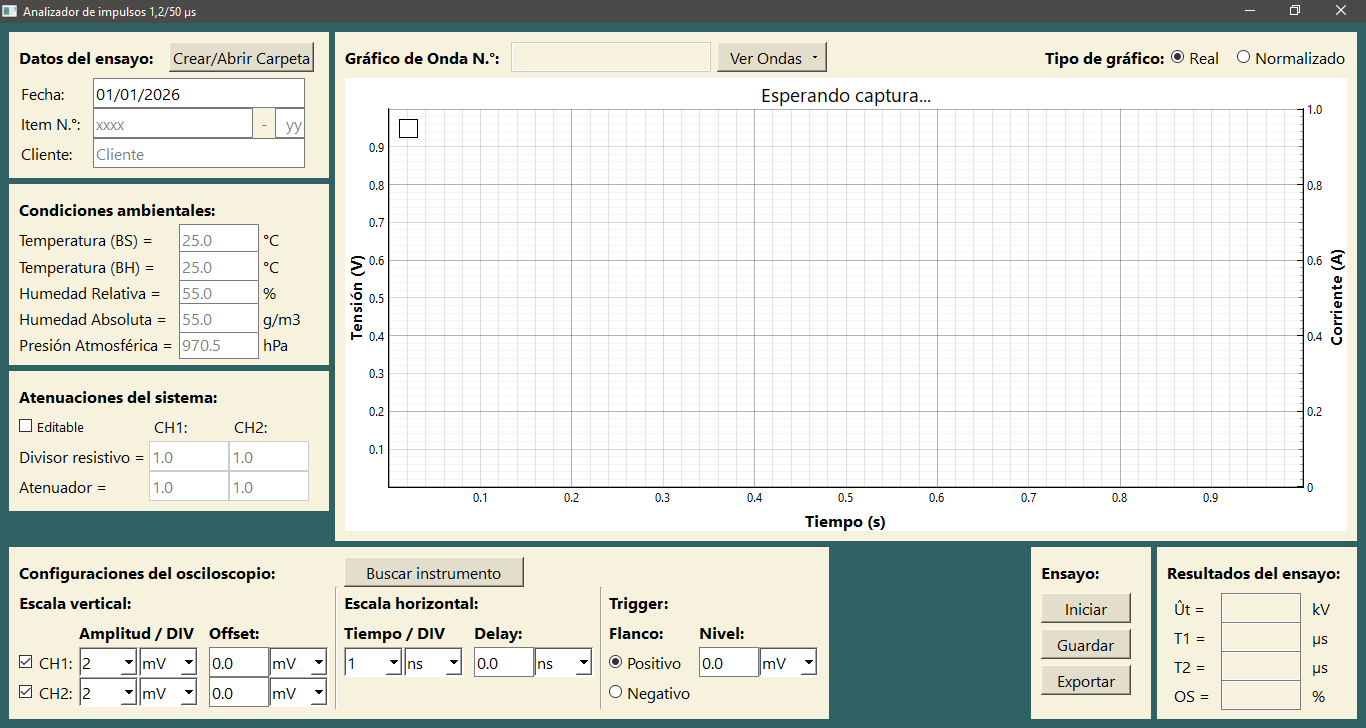
\includegraphics[width=1\textwidth]{img/GUI_1366x768.png}
    \caption{GUI en tamaño 1366x768 px.}
    \label{fig:GUI_1366x768}
\end{figure}

\begin{figure}[H]
    \centering
    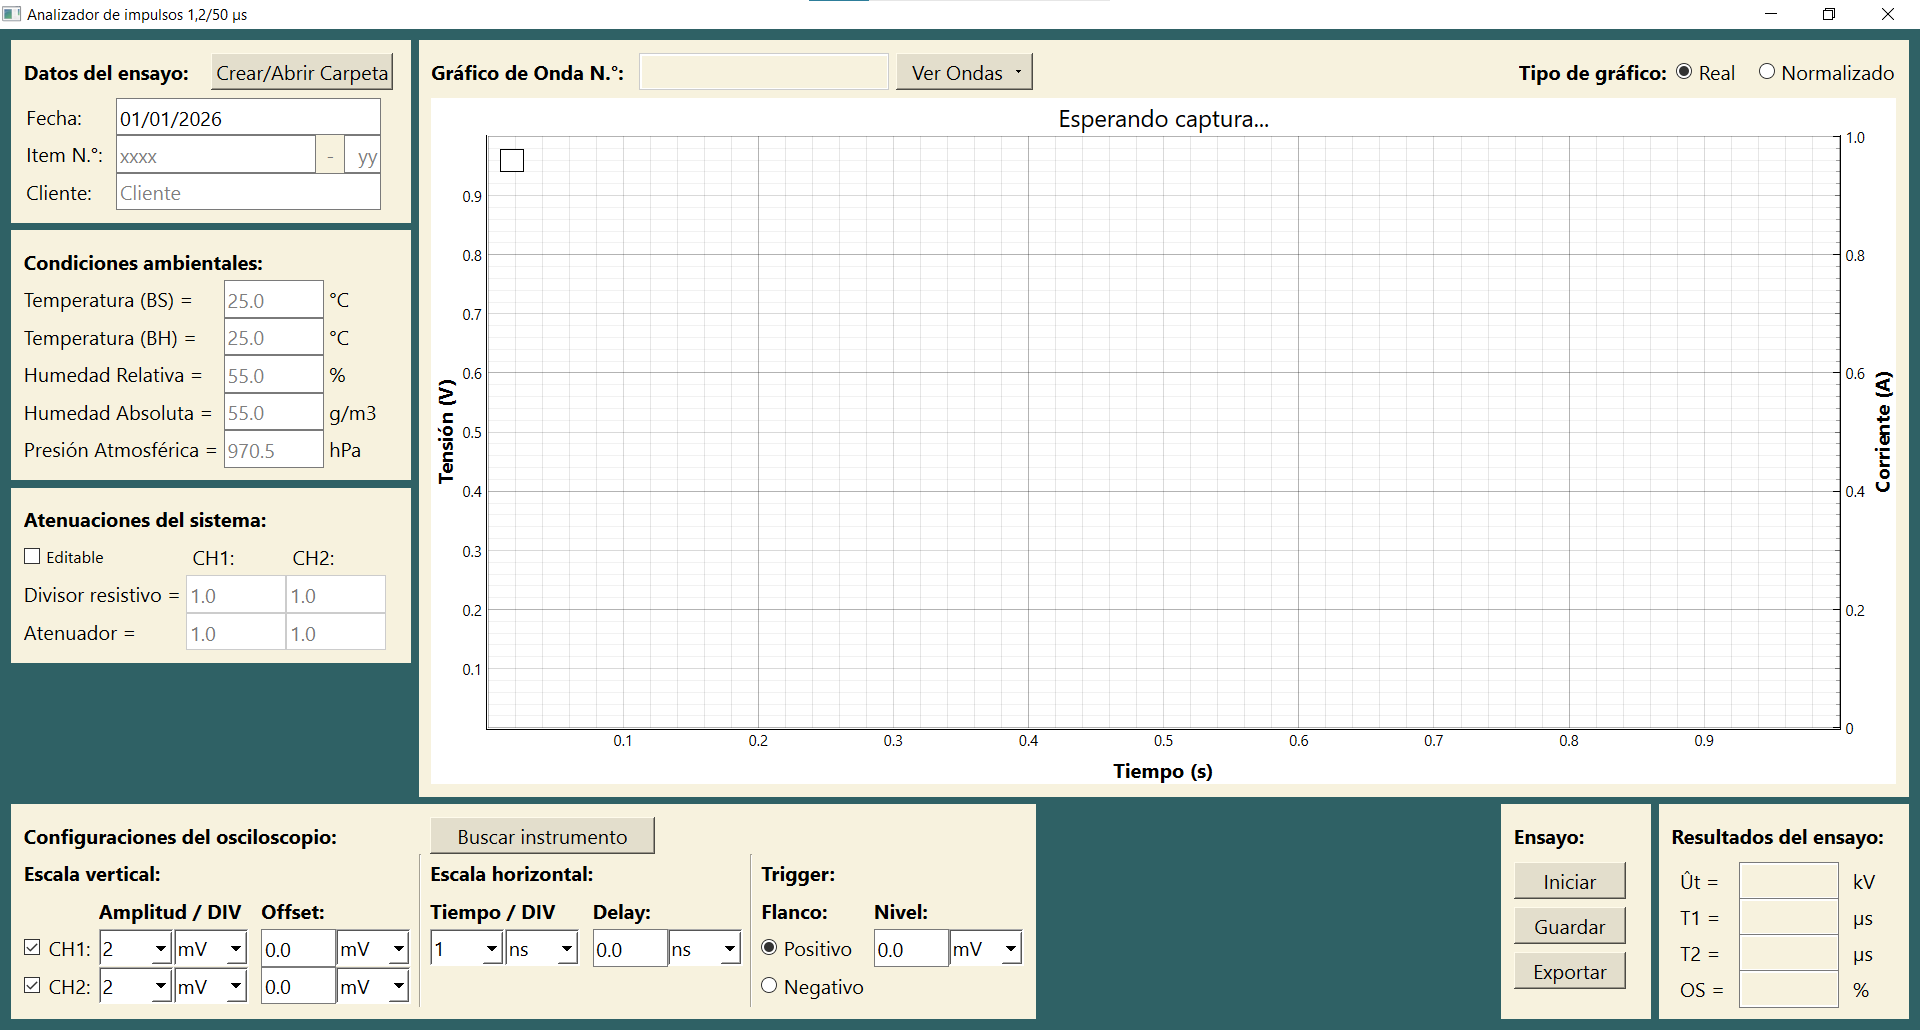
\includegraphics[width=1\textwidth]{img/GUI_1920x1080.png}
    \caption{GUI en tamaño 1920x1080 px.}
    \label{fig:GUI_1920x1080}
\end{figure}

\subsection{Diagramación de la GUI:}

Con el fin de que sea intuitivo para los operadores, se diseñó un recorrido lógico para trabajar en la ventana.

\begin{figure}[H]
    \centering
    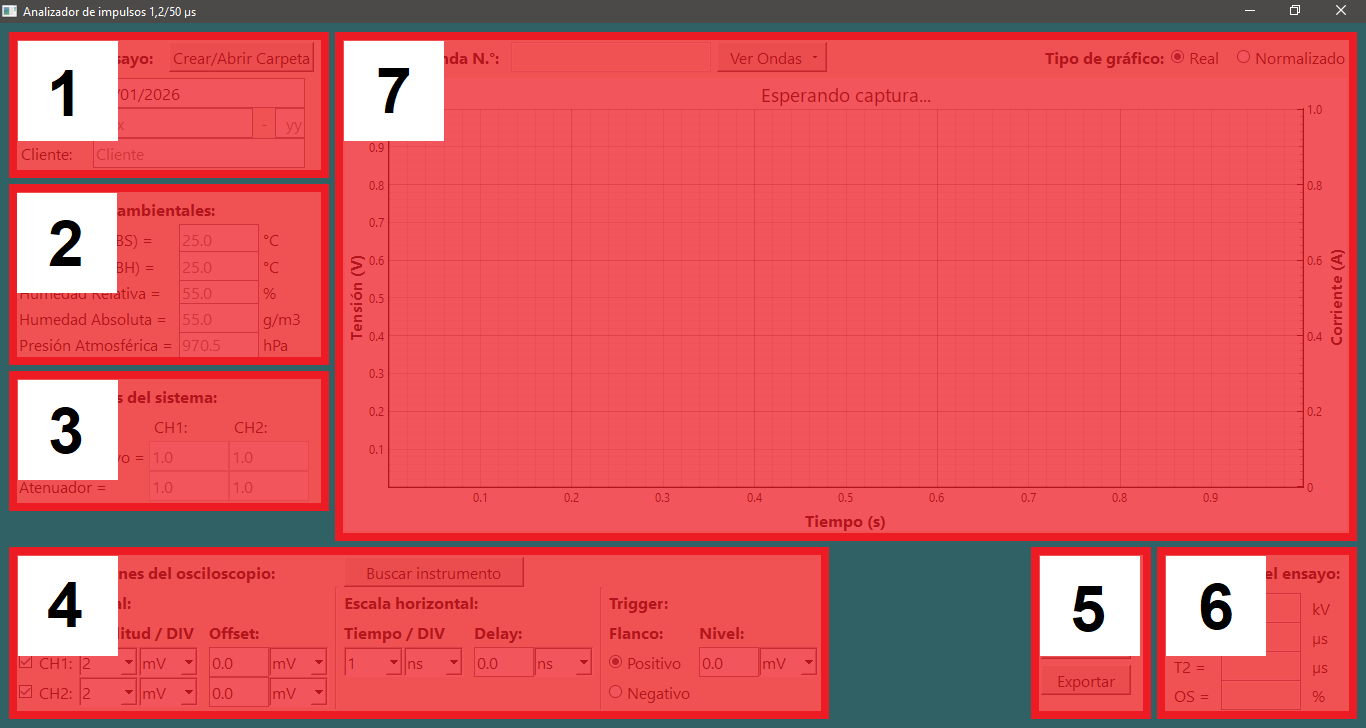
\includegraphics[width=1\textwidth]{img/GUI_Bloques.png}
    \caption{Flujo de trabajo.}
    \label{fig:recorrido_gui}
\end{figure}

\begin{enumerate}
    \item \textbf{Datos del ensayo}: Sirve para cargar los datos relacionados a la trazabilidad del laboratorio sobre del elemento que se va a ensayar.
    \begin{figure}[H]
        \centering
        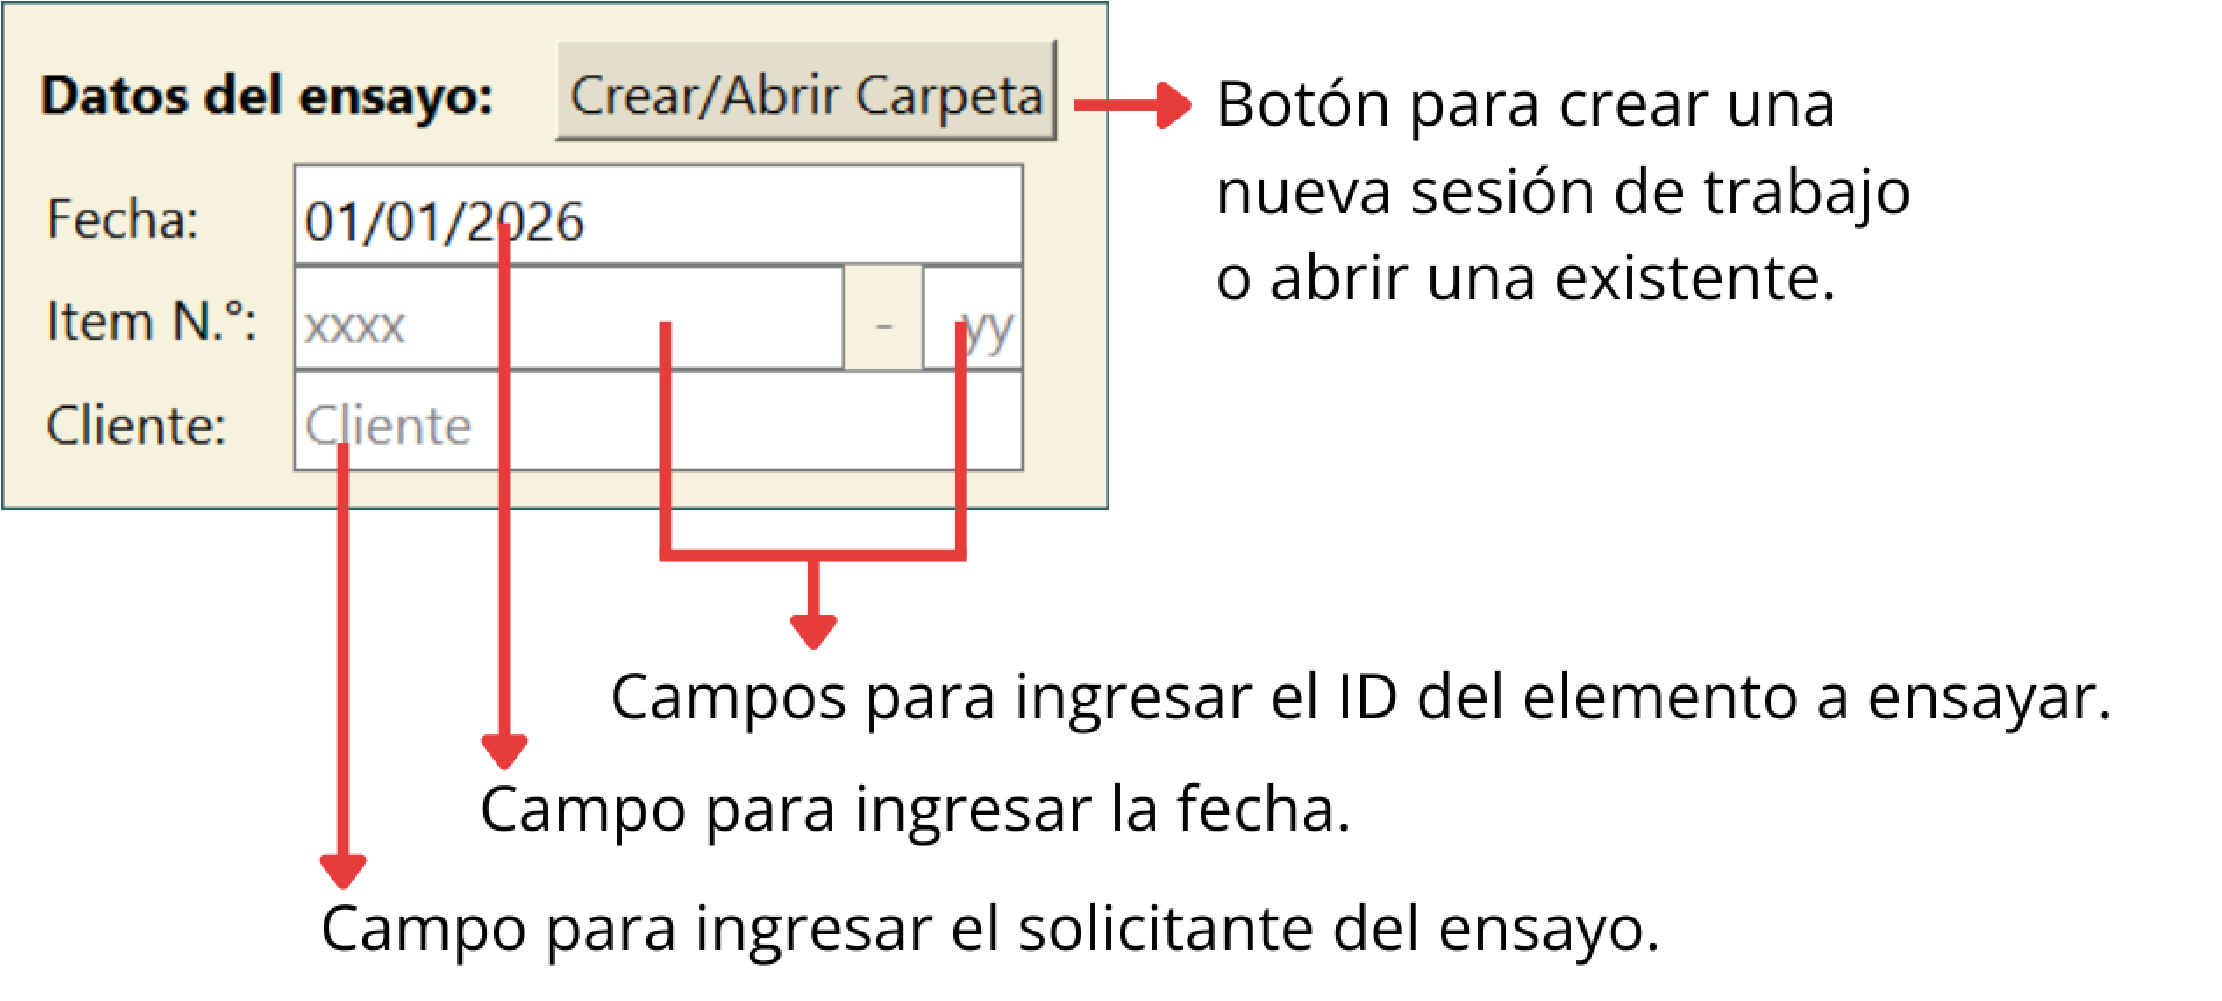
\includegraphics[width=0.8\textwidth]{img/GUI_1_datos_ensayo.png}
        \caption{Bloque de Datos de ensayo.}
        \label{fig:GUI_1_Datos_ensayo}
    \end{figure}
    \item \textbf{Condiciones ambientales}: Donde el operador introduce parámetros termodinámicos de referencia como la temperatura, presión y humedad. Estos valores son esenciales para la posterior corrección atmosférica de la tensión de ensayo $U_t$ de acuerdo con la norma \textbf{IEC 60060-1} \cite{iec60060_1}.
    \begin{figure}[H]
        \centering
        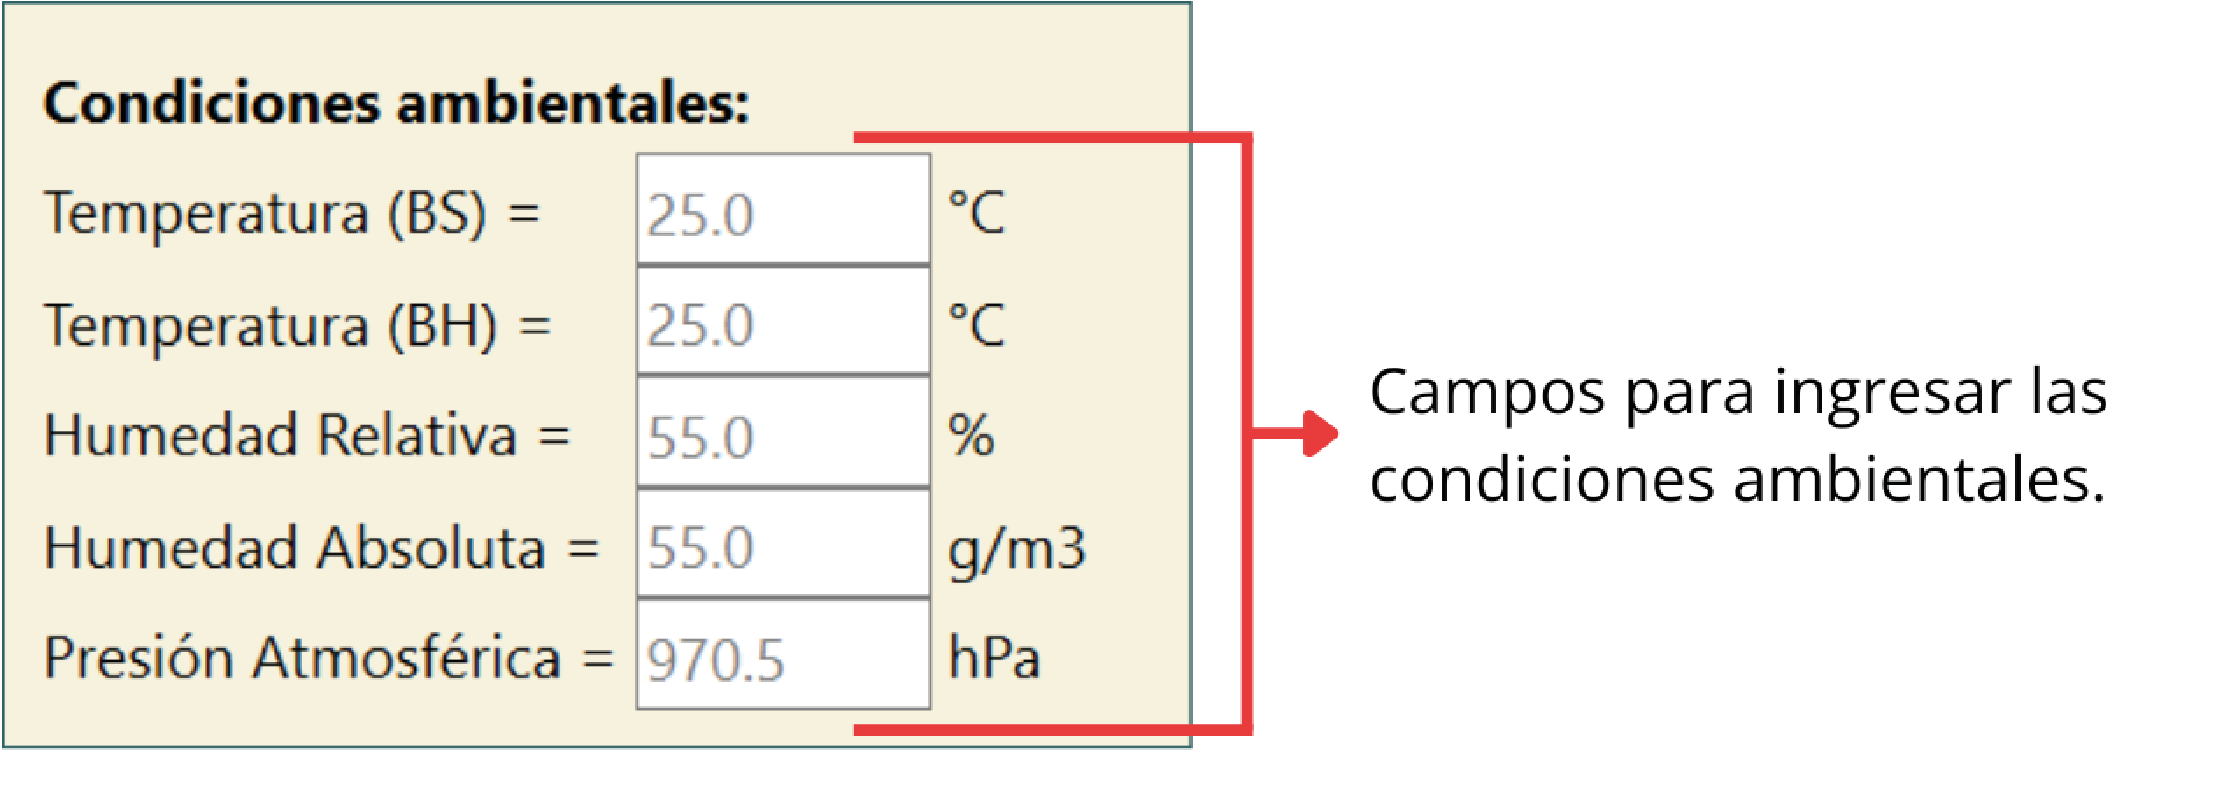
\includegraphics[width=0.8\textwidth]{img/GUI_2_condiciones_ambientales.png}
        \caption{Bloque de Condiciones ambientales.}
        \label{fig:GUI_2_condiciones_ambientales}
    \end{figure}
    \item \textbf{Atenuaciones del sistema}: Para ingresar los factores de atenuación de los divisores resistivos y atenuadores coaxiales, correspondientes al sistema de medición.
    \begin{figure}[H]
        \centering
        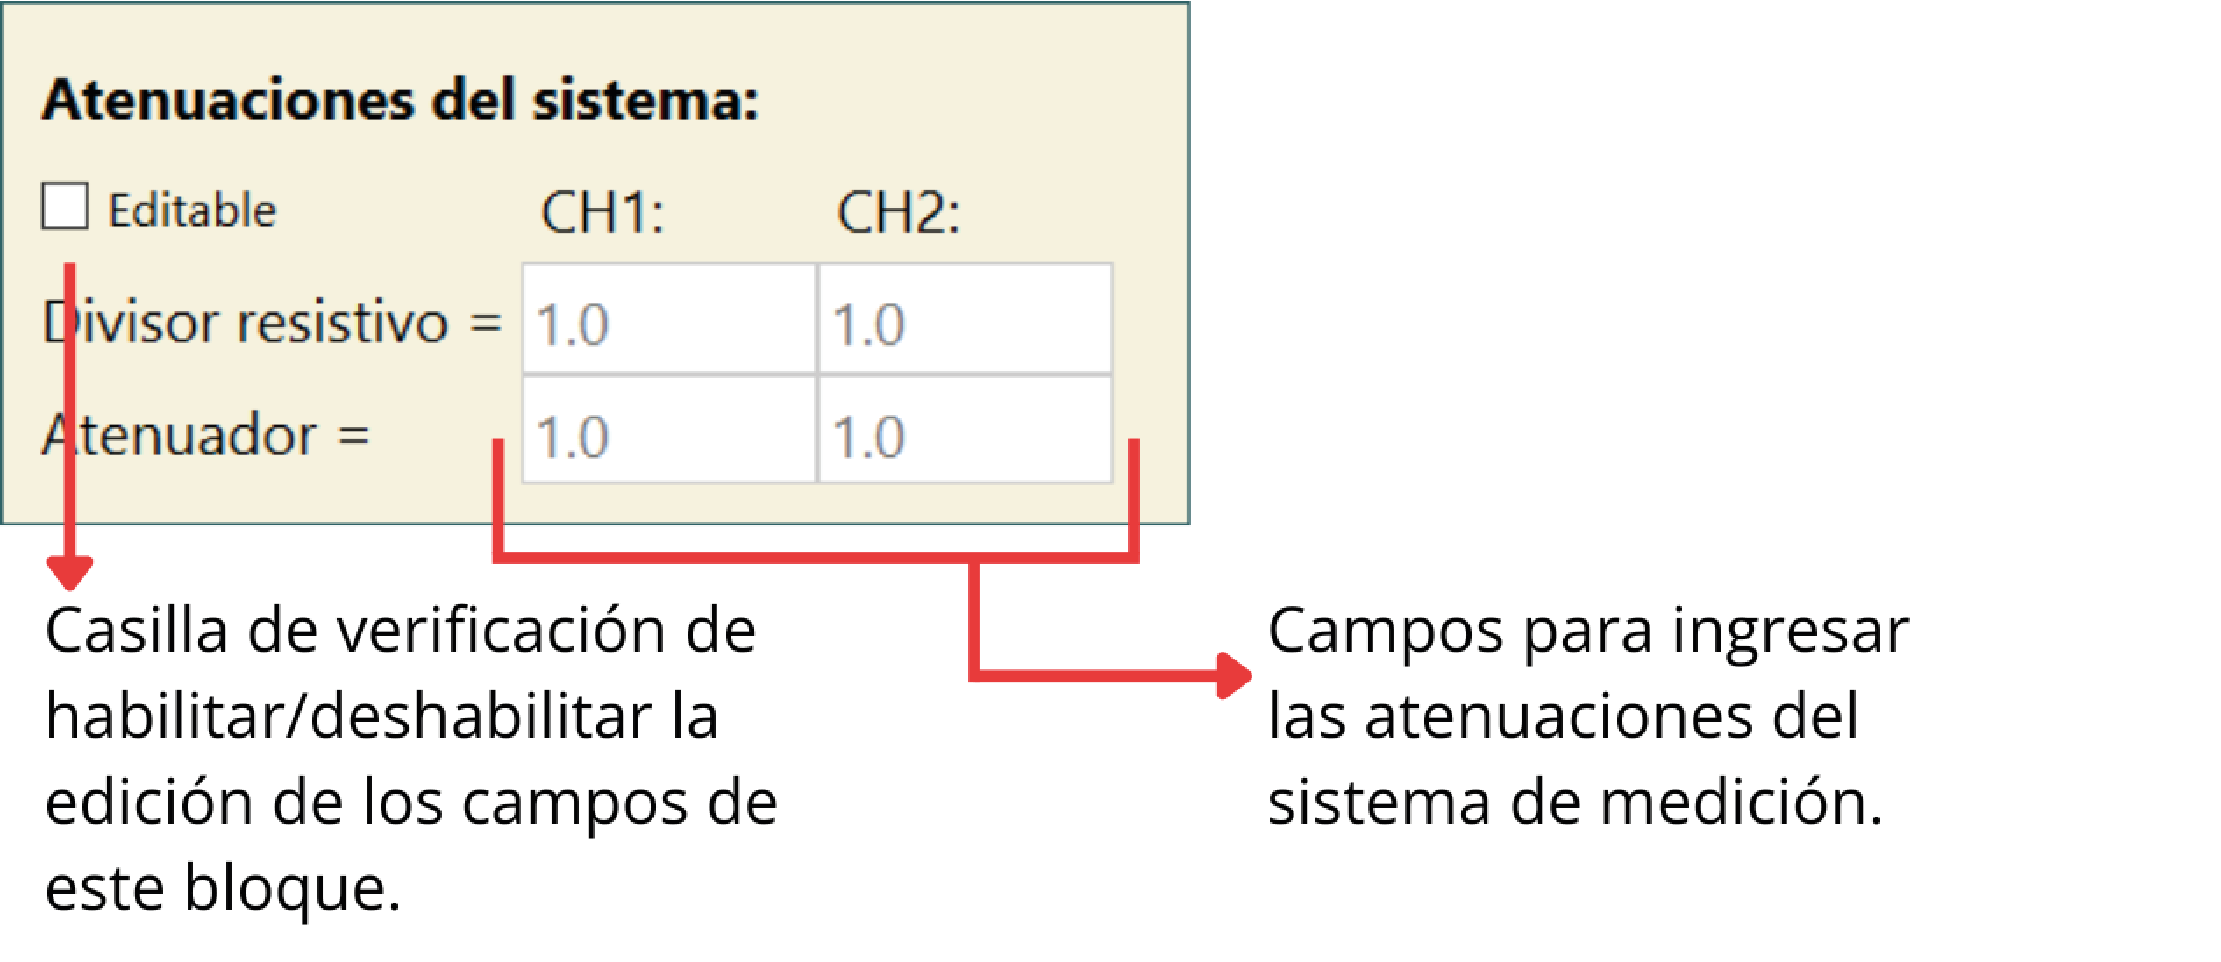
\includegraphics[width=0.8\textwidth]{img/GUI_3_atenuaciones.png}
        \caption{Bloque de Atenuaciones del sistema de medición.}
        \label{fig:GUI_3_atenuaciones}
    \end{figure}
    \item \textbf{Configuraciones del osciloscopio}: Agrupa los comandos de control del instrumento
    \begin{figure}[H]
        \centering
        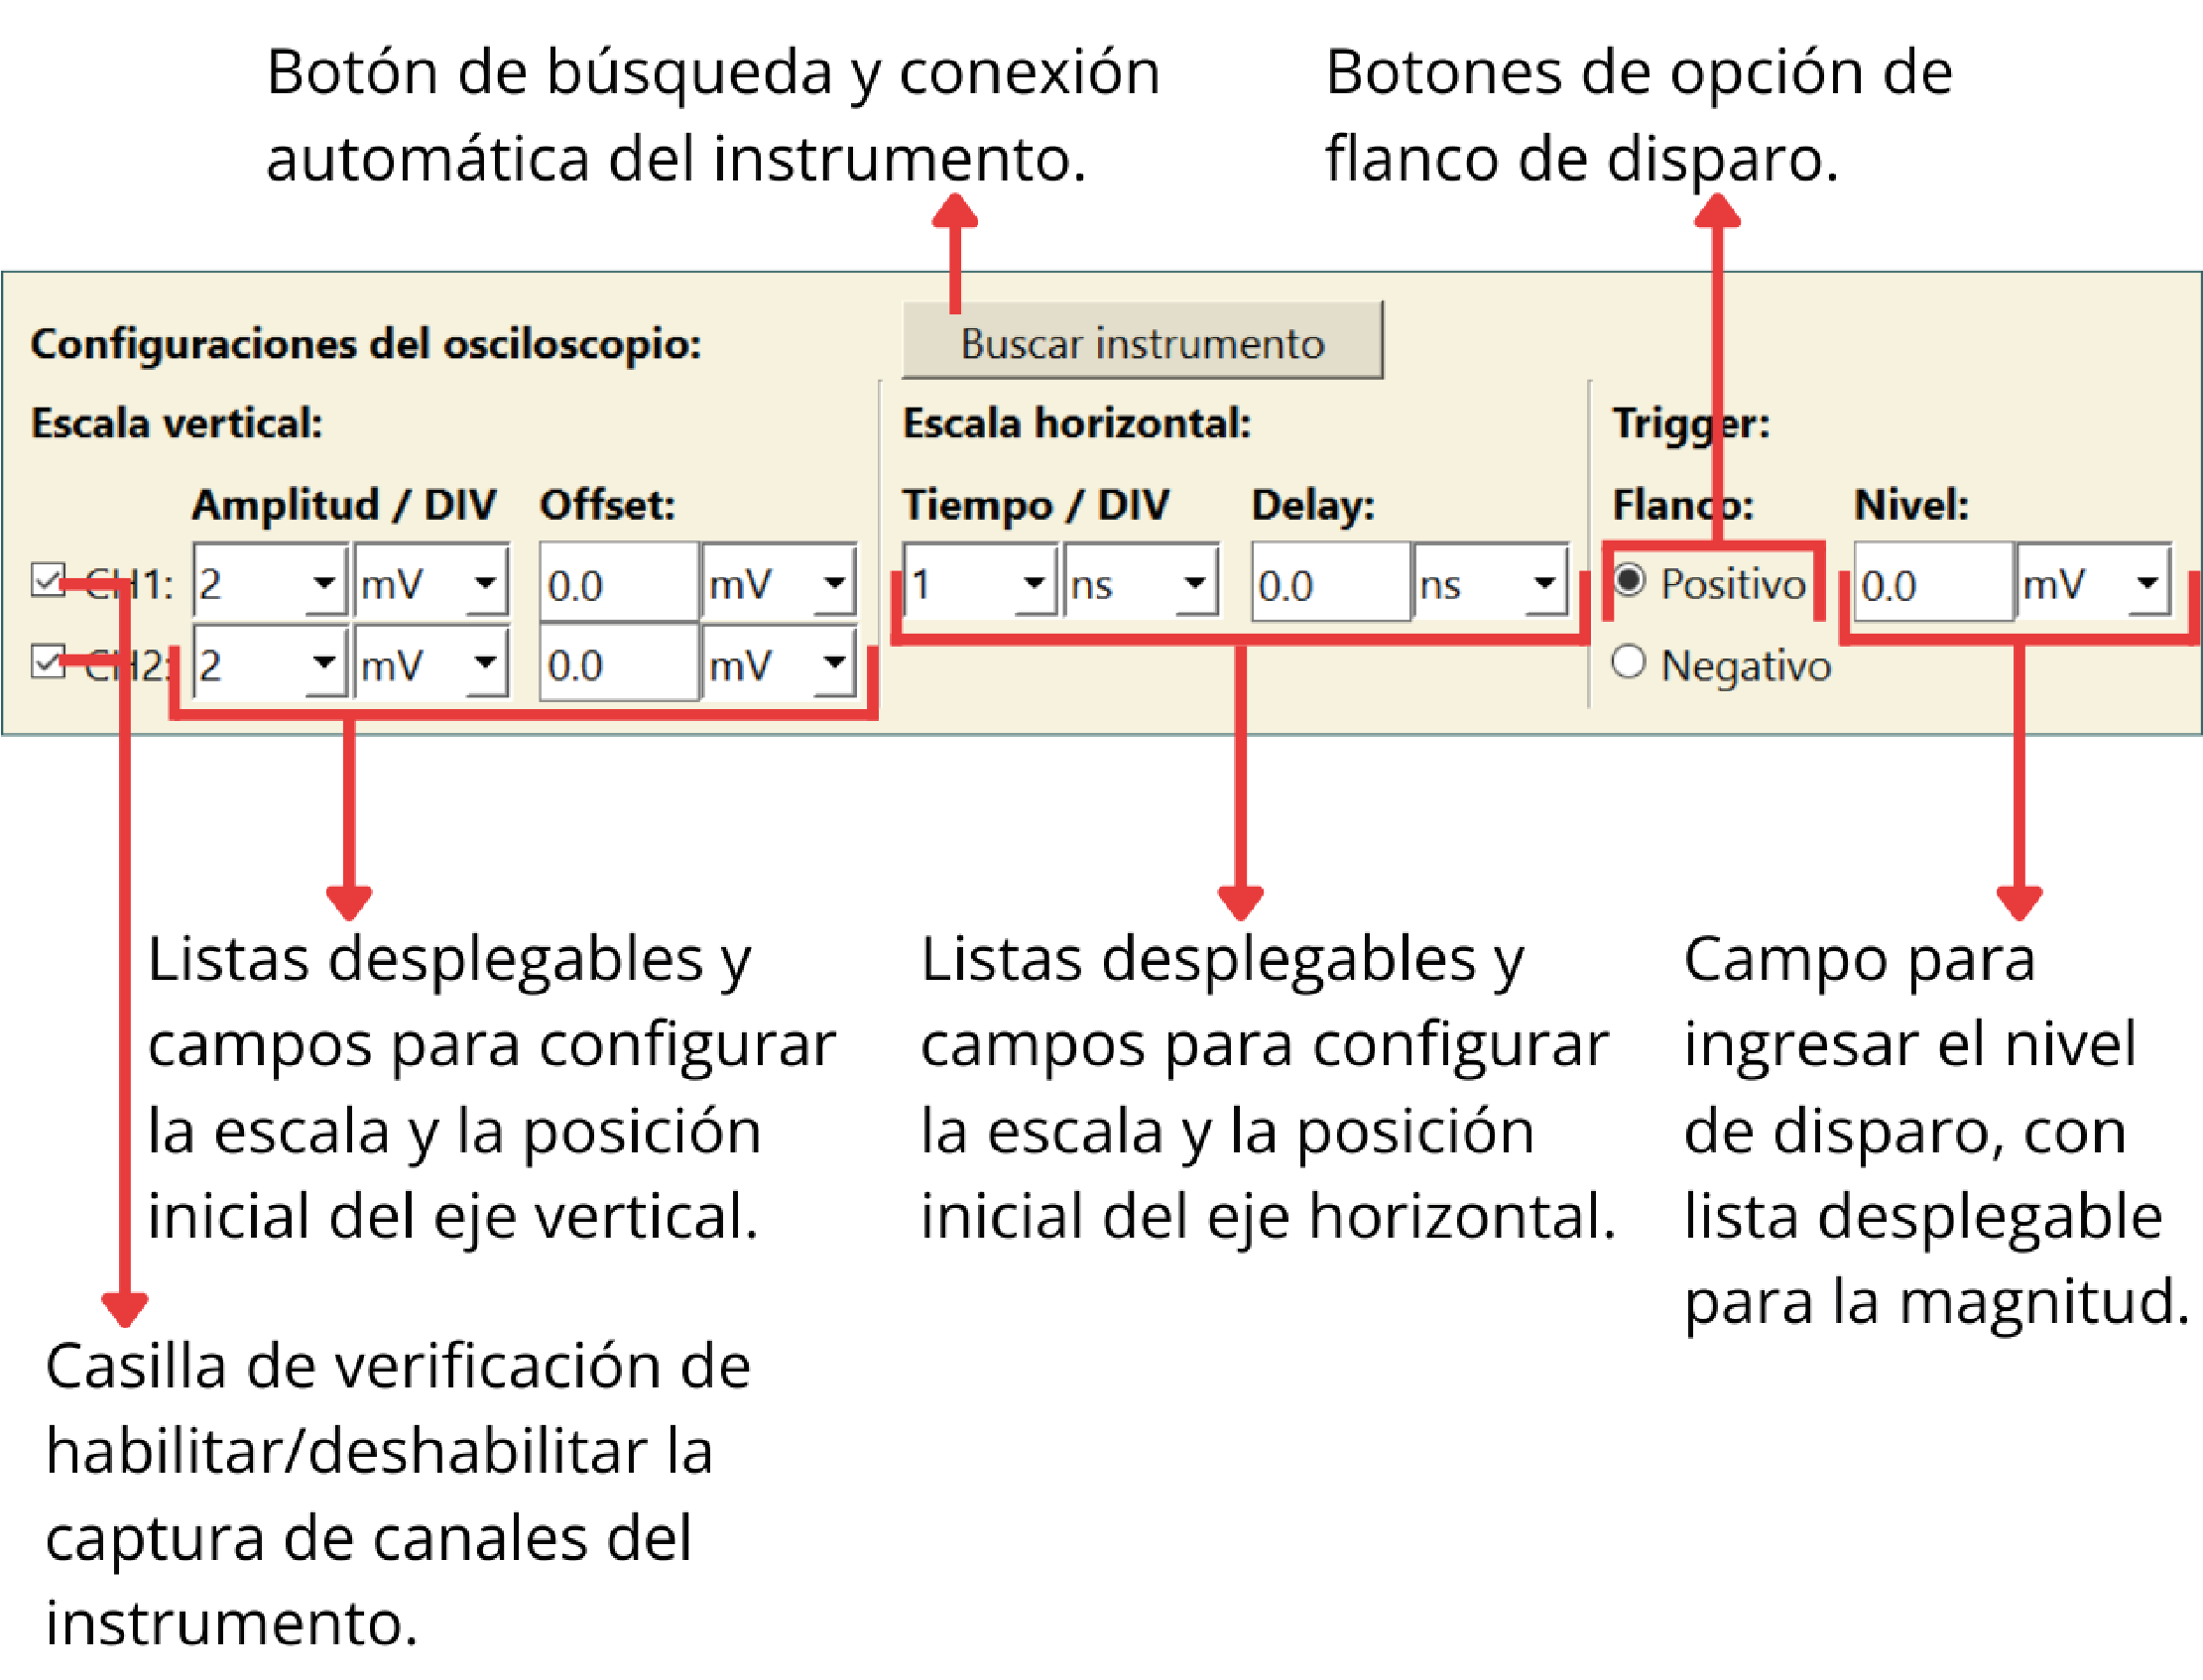
\includegraphics[width=1\textwidth]{img/GUI_4_control_osciloscopio.png}
        \caption{Bloque de Control del instrumento.}
        \label{fig:GUI_4_control_osciloscopio}
    \end{figure}
    \item \textbf{Ensayo}: Permite al usuario ejecutar la adquisición de señal, guardar los registros en la base de datos y realizar la exportación en formatos planos como Excel o CSV.
    \begin{figure}[H]
        \centering
        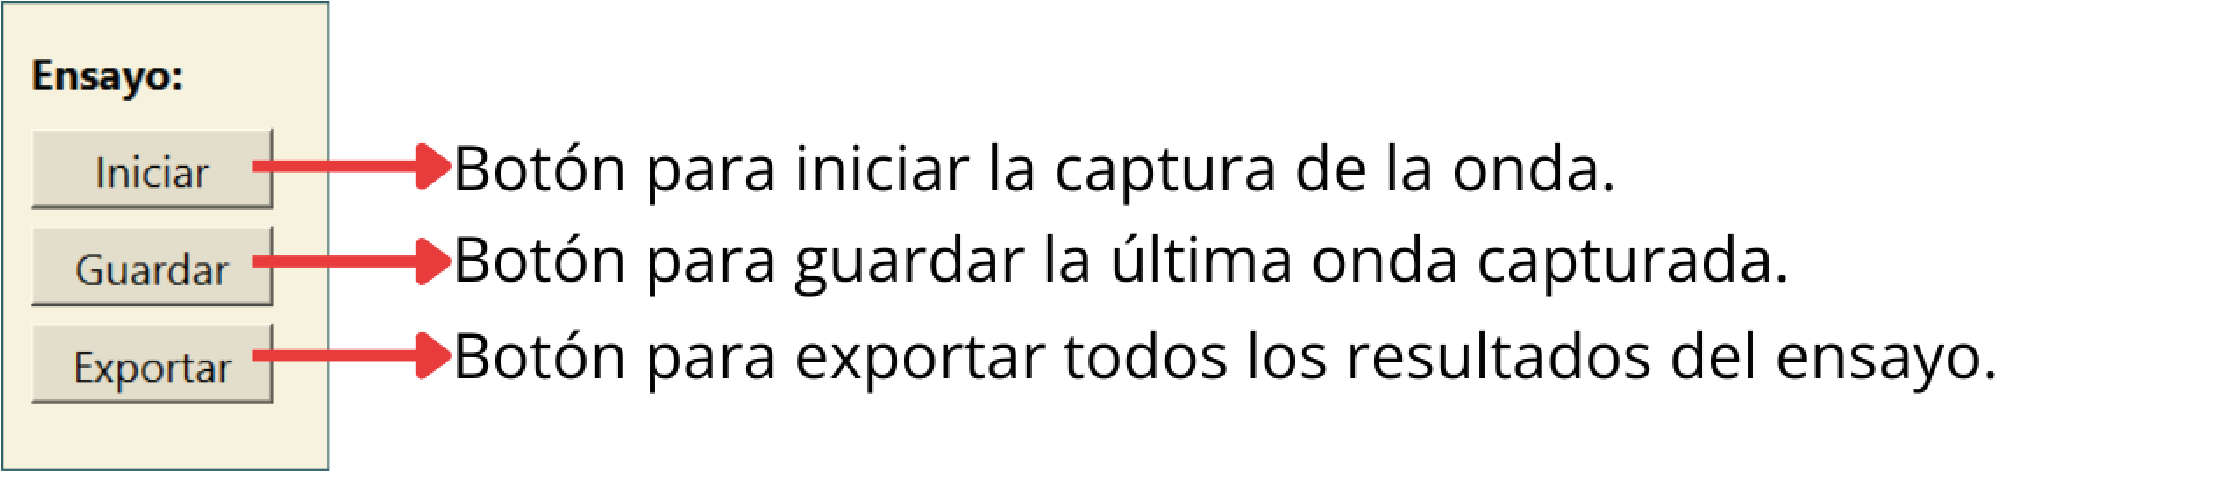
\includegraphics[width=0.8\textwidth]{img/GUI_5_opciones_ensayo.png}
        \caption{Bloque de Opciones de ensayo.}
        \label{fig:GUI_5_opciones_ensayo}
    \end{figure}
    \item \textbf{Resultados del ensayo}: Este panel renderiza dinámicamente en una tabla los parámetros de la onda calculados tras la adquisición ($U_t$, $T_1$, $T_2$ o $T_c$ y $OS\%$).
    \begin{figure}[H]
        \centering
        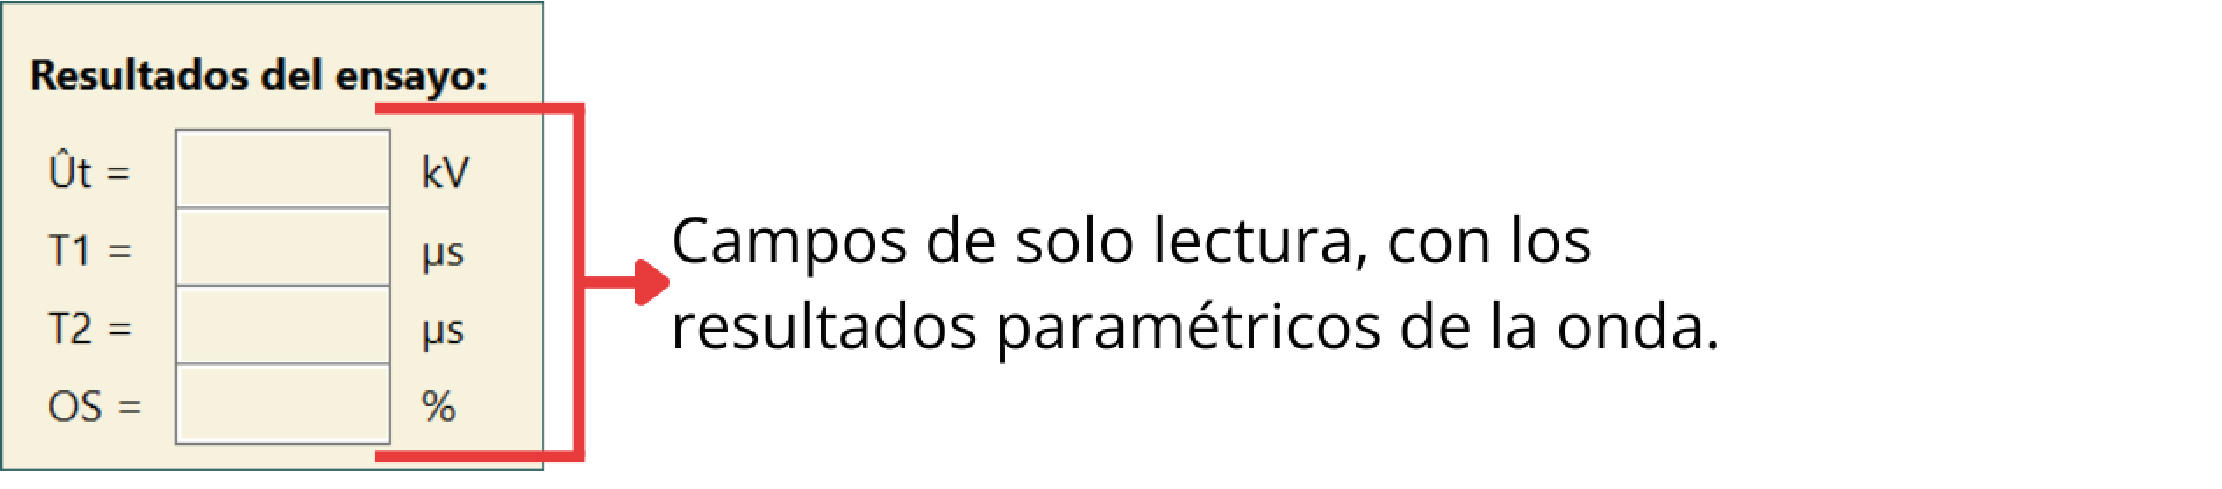
\includegraphics[width=0.8\textwidth]{img/GUI_6_resultados_ensayo.png}
        \caption{Bloque de Resultados de ensayo.}
        \label{fig:GUI_6_resultados_ensayo}
    \end{figure}
    \item \textbf{Gráfico de ondas}: El área de mayor tamaño de la pantalla se reservó para el renderizado de las curvas de tensión y corriente.
    \begin{figure}[H]
        \centering
        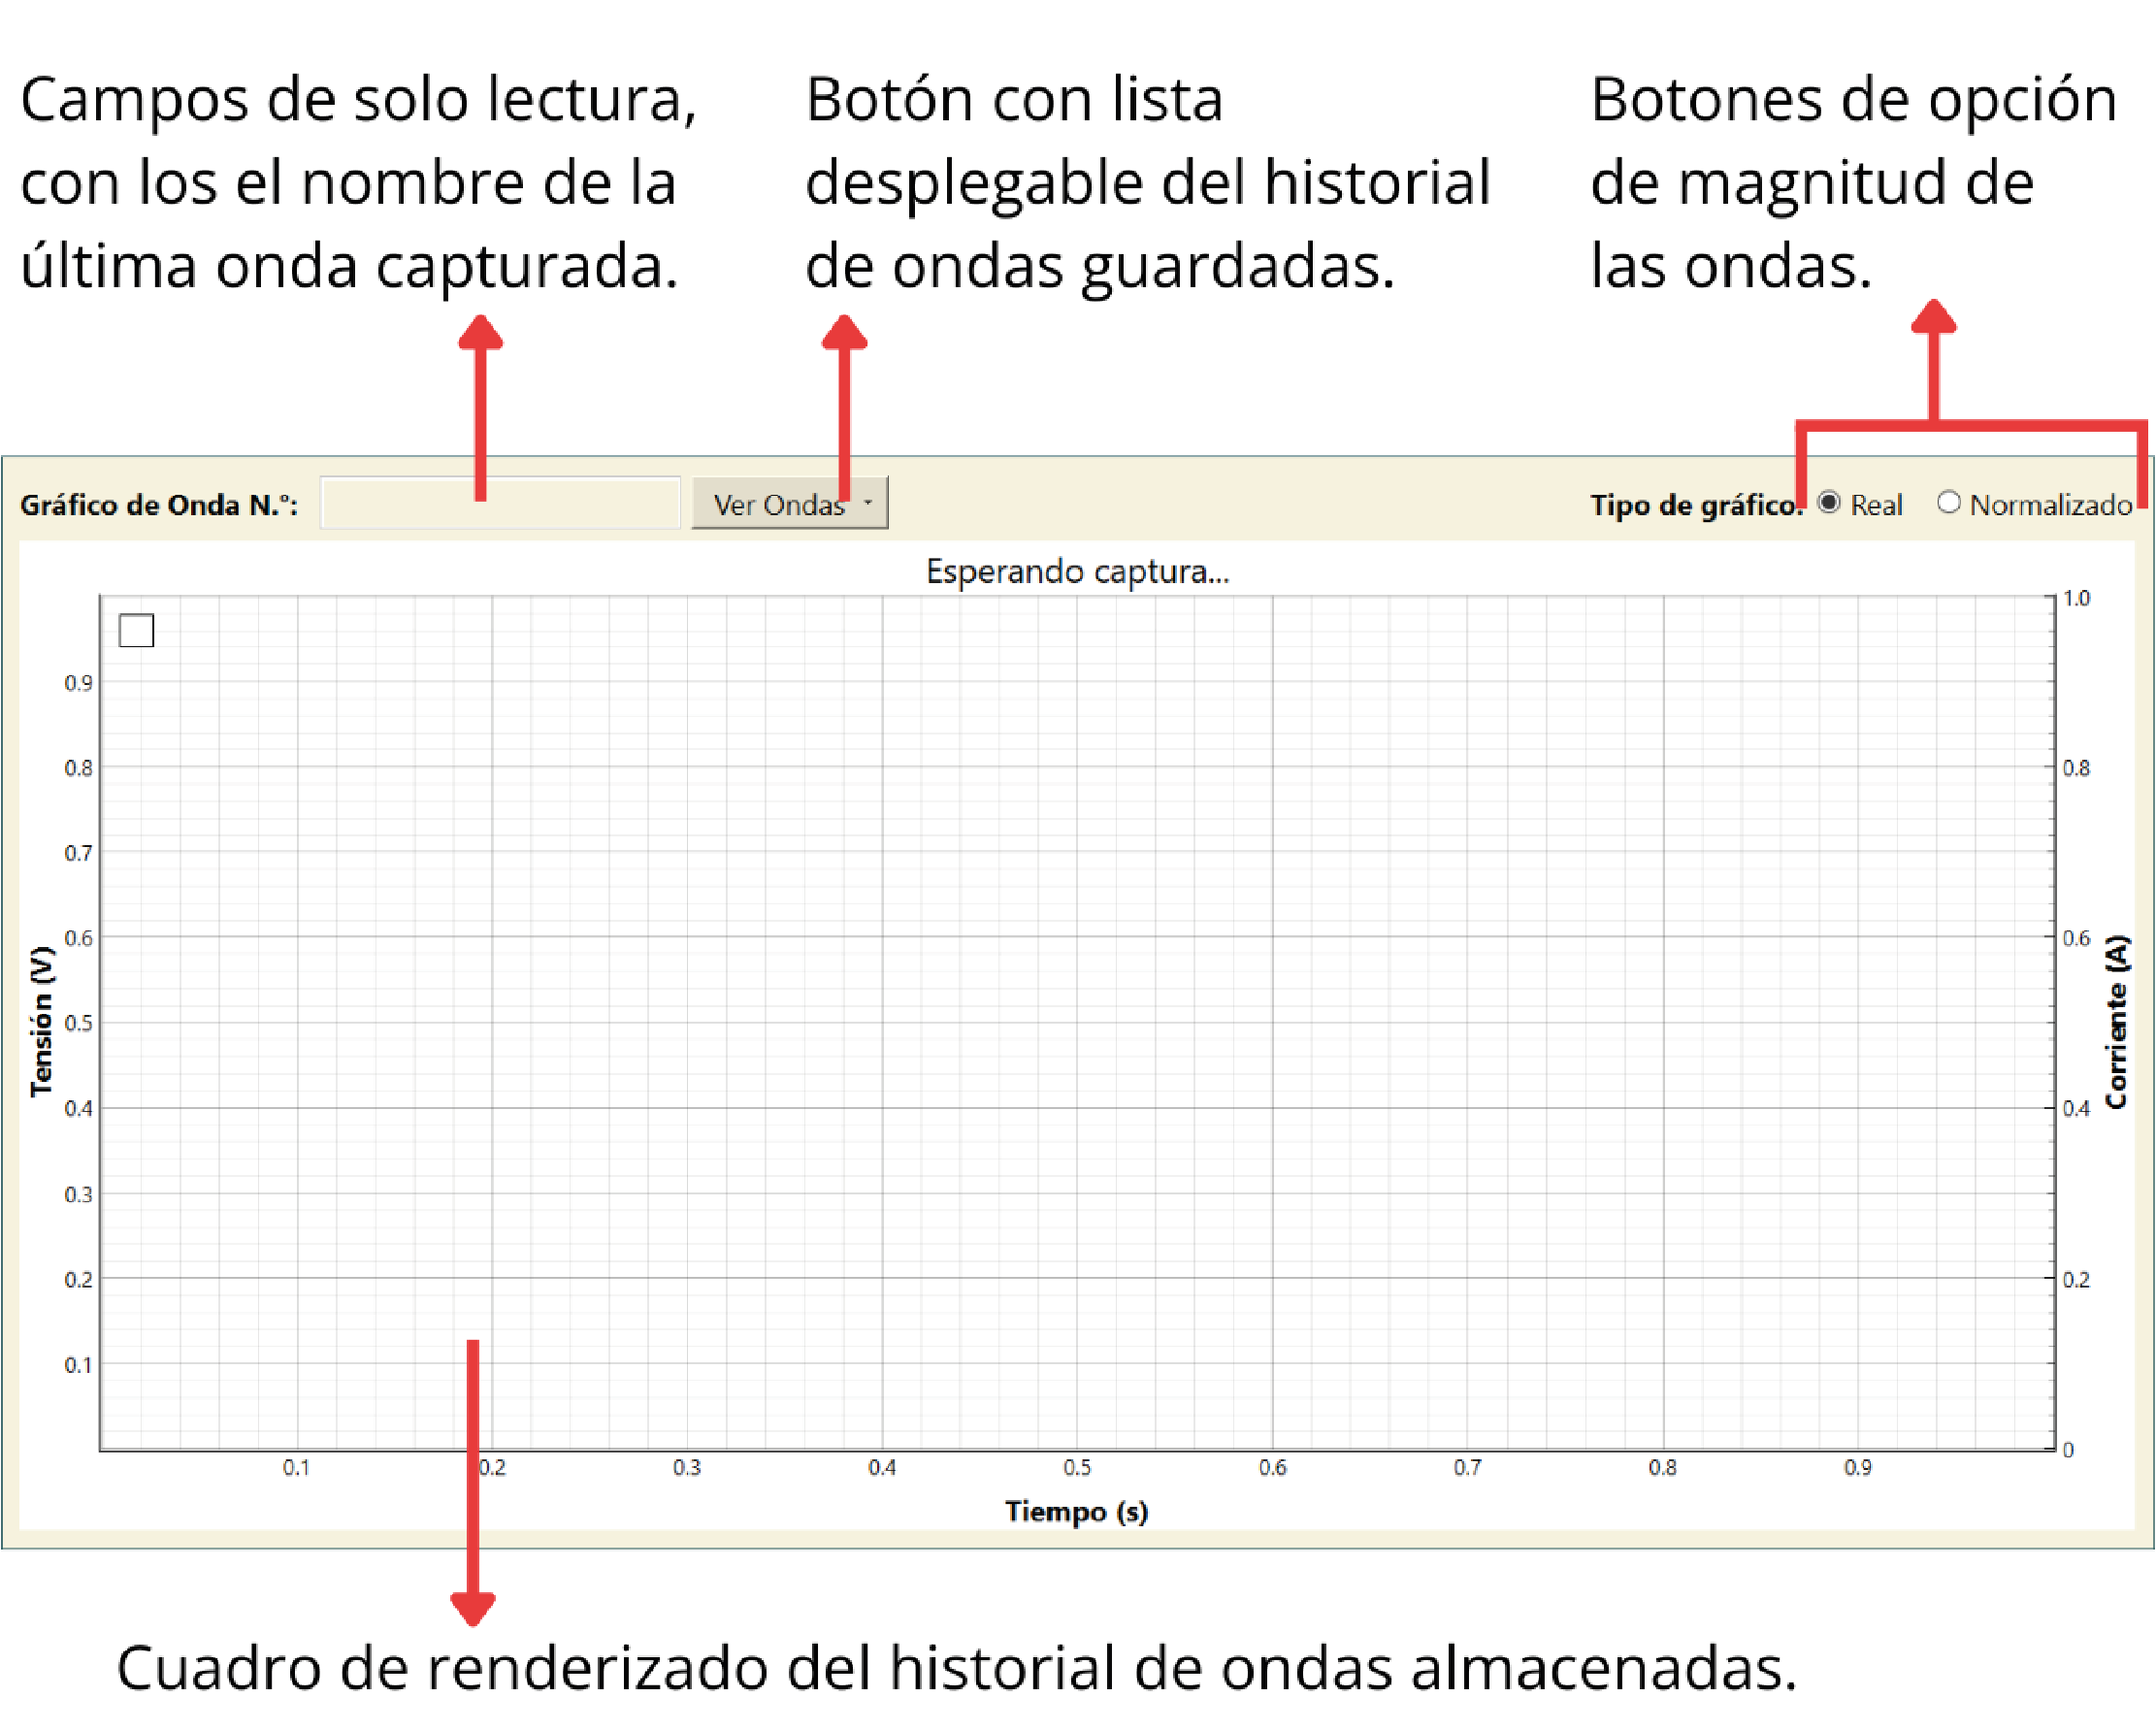
\includegraphics[width=1\textwidth]{img/GUI_7_grafico.png}
        \caption{Bloque de Gráfico.}
        \label{fig:GUI_7_grafico}
    \end{figure}
\end{enumerate}

\subsection{Guía de uso}

A modo de ejemplo se presenta a continuación, una guía paso a paso del flujo de trabajo a realizar por el operario, desde que inicia el programa hasta que exporta los resultados.

\begin{enumerate}
    \begin{figure}[H]
        \centering
        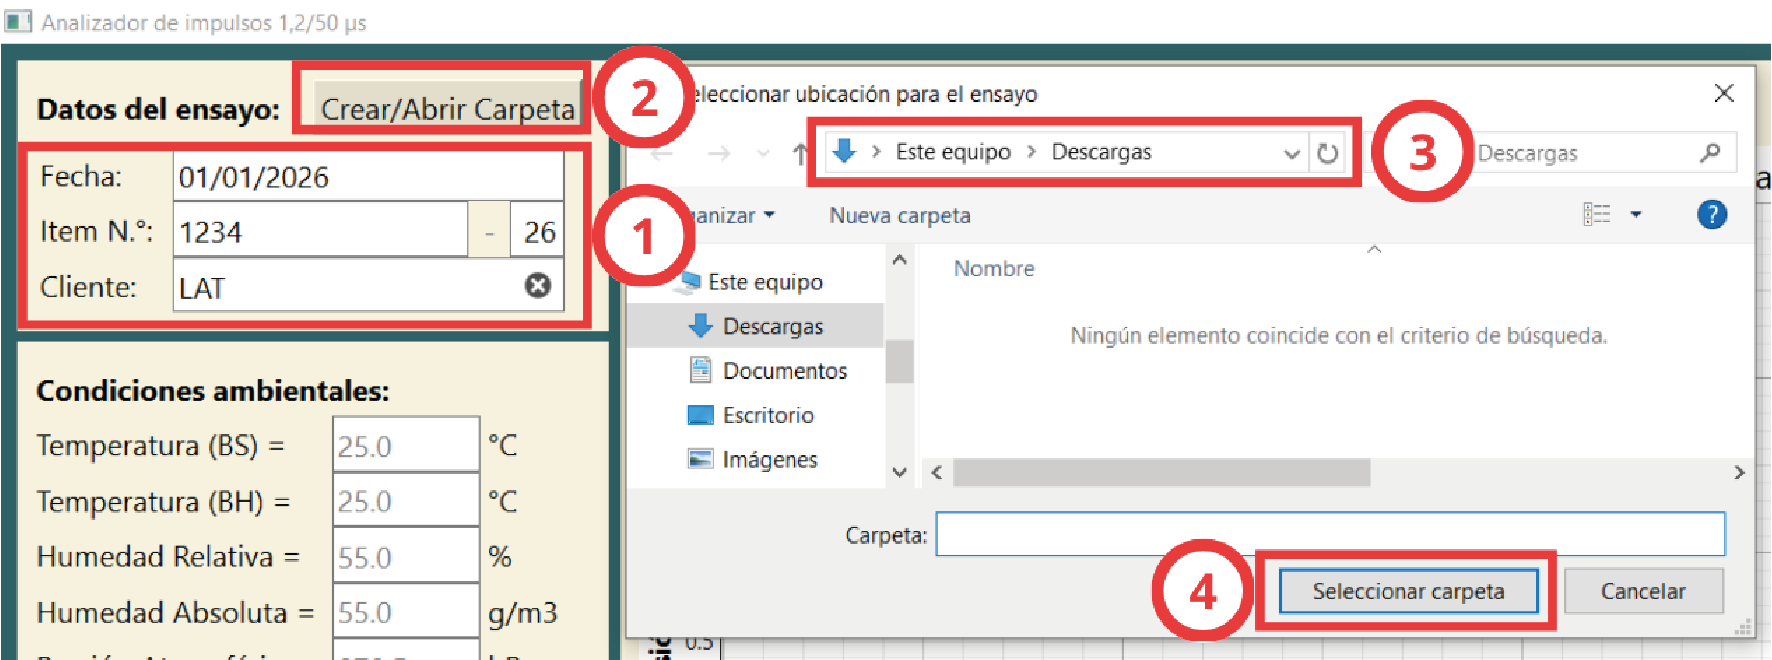
\includegraphics[width=1\textwidth]{img/GUI_uso_1_crear_sesion.png}
        \caption{Creación de directorio del ensayo.}
        \label{fig:GUI_uso_1_crear_sesion}
    \end{figure}
    \item [\textbf{Paso 1:}] Completar los campos del elemento a ensayar.
    \item [\textbf{Paso 2:}] Accionar el botón \enquote{Crear/Abrir Carpeta} para crear una nueva carpeta.
    \item [\textbf{Paso 3:}] Buscar la ruta donde se creará la carpeta.
    \item [\textbf{Paso 4:}] Crear la carpeta.
    \begin{figure}[H]
        \centering
        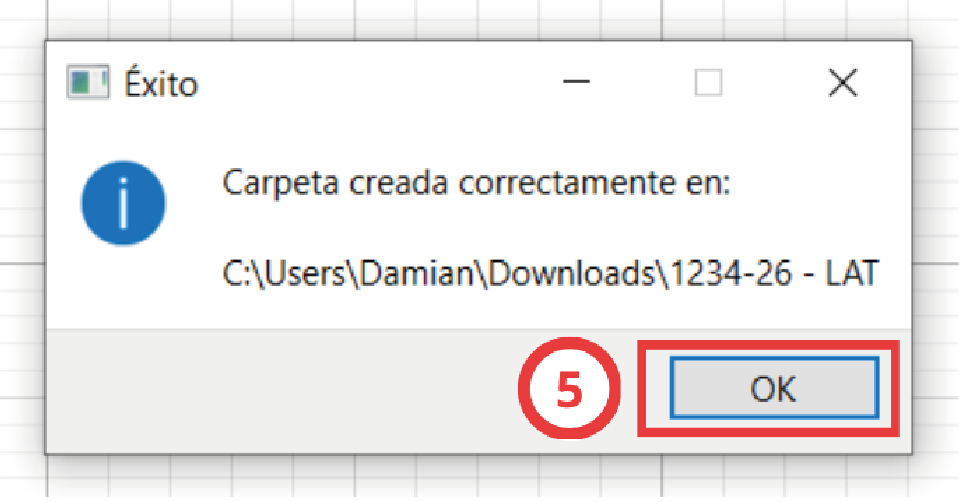
\includegraphics[width=0.5\textwidth]{img/GUI_uso_2_sesion_creada.png}
        \caption{Notificación de creación de carpeta exitosa.}
        \label{fig:GUI_uso_2_sesion_creada}
    \end{figure}
    \item [\textbf{Paso 5:}] Confirmar que se creó correctamente la carpeta del ensayo.
    \begin{figure}[H]
        \centering
        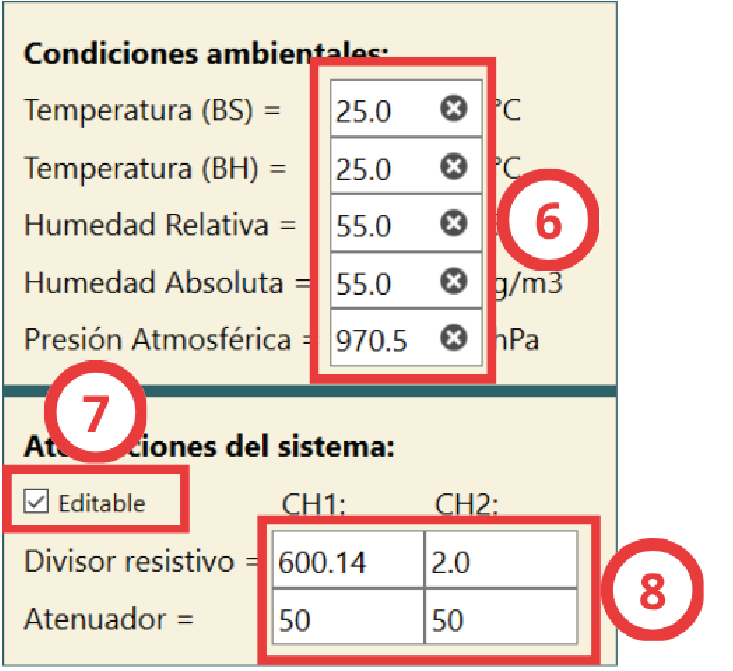
\includegraphics[width=0.5\textwidth]{img/GUI_uso_3_cargar_condiciones.png}
        \caption{Edición de campos a completar.}
        \label{fig:GUI_uso_3_cargar_condiciones}
    \end{figure}
    \item [\textbf{Paso 6:}] Cargar las condiciones ambientales.
    \item [\textbf{Paso 7:}] Habilitar (tildar) la edición de los campos de las atenuaciones.
    \item [\textbf{Paso 8:}] Completar los campos de las atenuaciones.
    \begin{figure}[H]
        \centering
        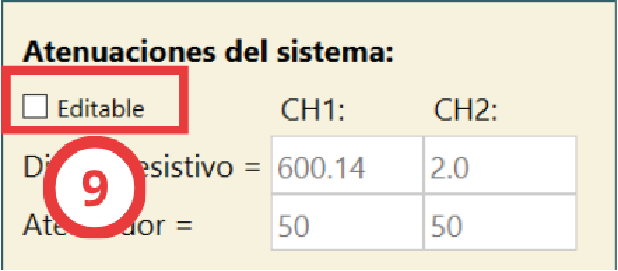
\includegraphics[width=0.5\textwidth]{img/GUI_uso_4_deshabilitar_atenuaciones.png}
        \caption{Deshabilitación de edición de campos de atenuaciones.}
        \label{fig:GUI_uso_4_deshabilitar_atenuaciones}
    \end{figure}
    \item [\textbf{Paso 9:}] Deshabilitar (destildar) la edición de los campos de las atenuaciones.
    \begin{figure}[H]
        \centering
        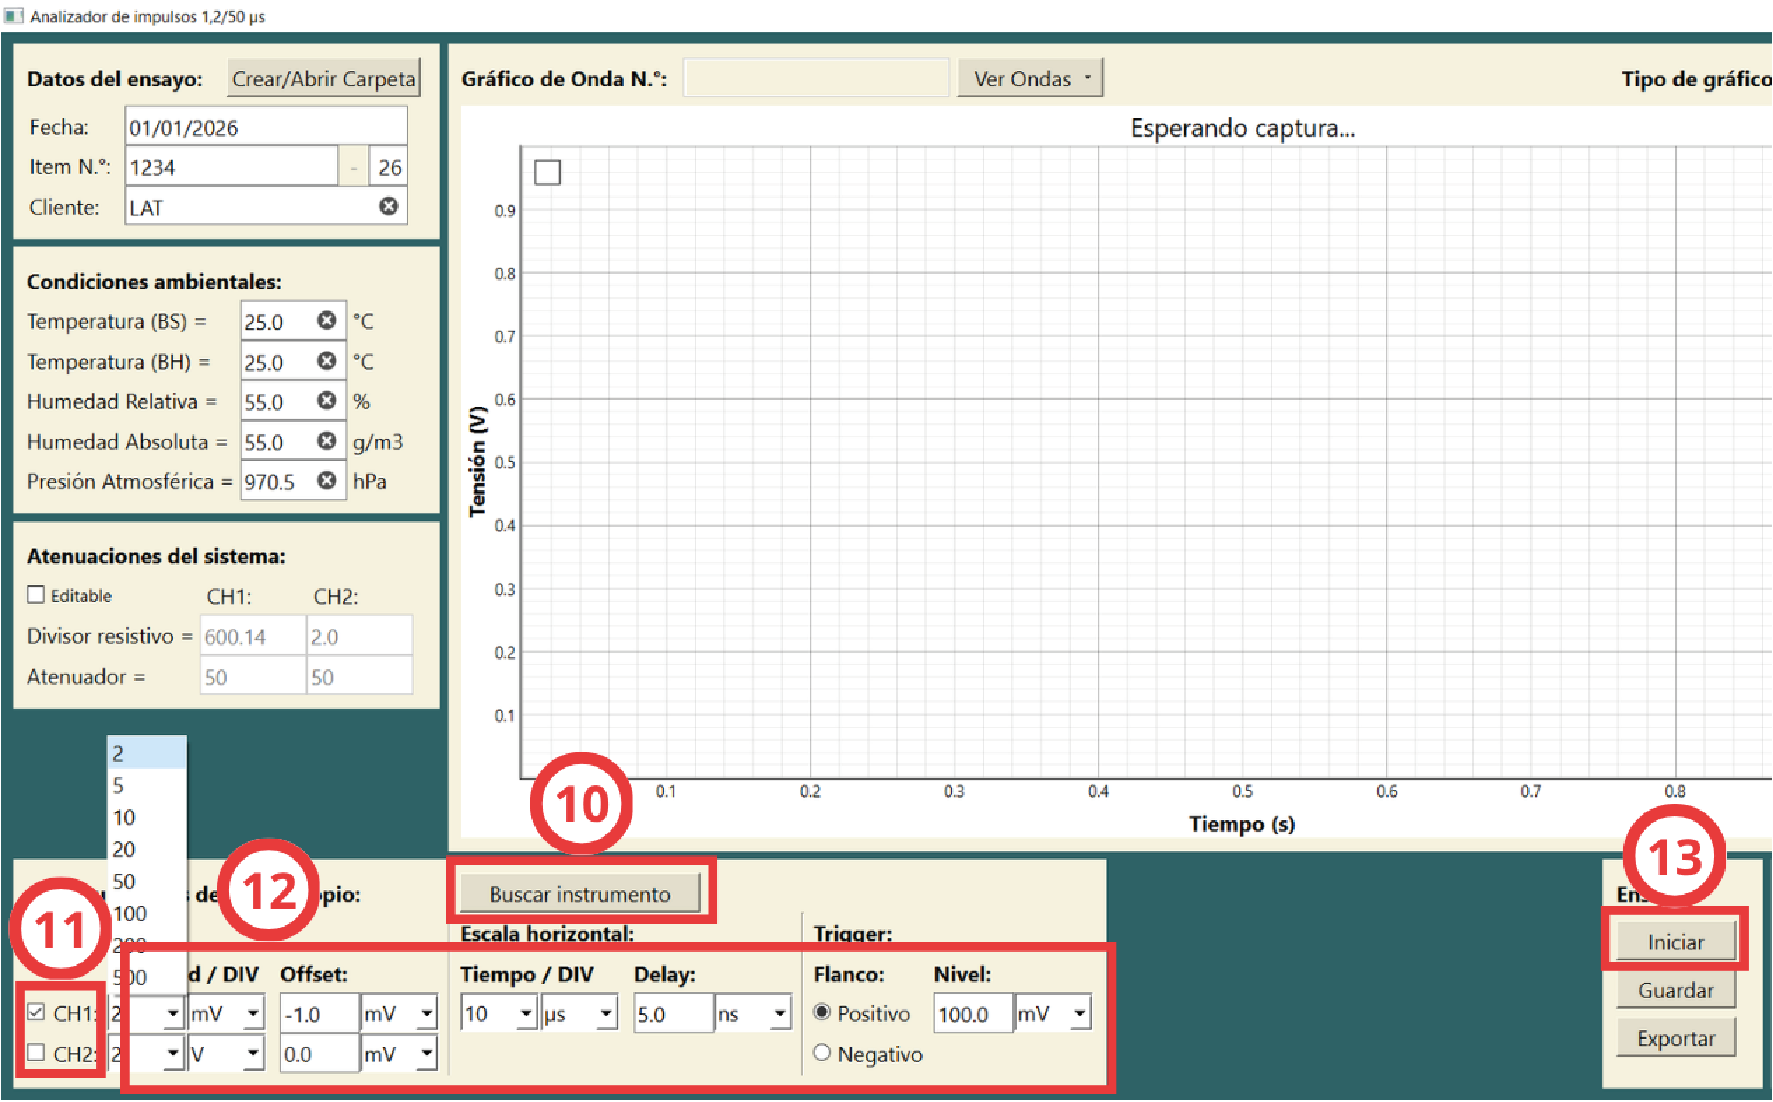
\includegraphics[width=1\textwidth]{img/GUI_uso_5_configurar_instrumento.png}
        \caption{Configuración del osciloscopio.}
        \label{fig:GUI_uso_5_configurar_instrumento}
    \end{figure}
    \item [\textbf{Paso 10:}] Conectar el osciloscopio a un puerto USB de la computadora y accionar el botón de búsqueda del instrumento. Cuando lo detecta, se conecta automáticamente.
    \emph{Nota: si conecta el instrumento antes de abrir el programa, se conectará automáticamente desde el inicio.}
    \item [\textbf{Paso 11:}] Habilitar/deshabilitar los canales del osciloscopio que se vayan a usar.
    \item [\textbf{Paso 12:}] Configurar los parámetros del osciloscopio.
    \item [\textbf{Paso 13:}] Accionar el botón \enquote{Iniciar} para comenzar la captura del impuslo.
    \begin{figure}[H]
        \centering
        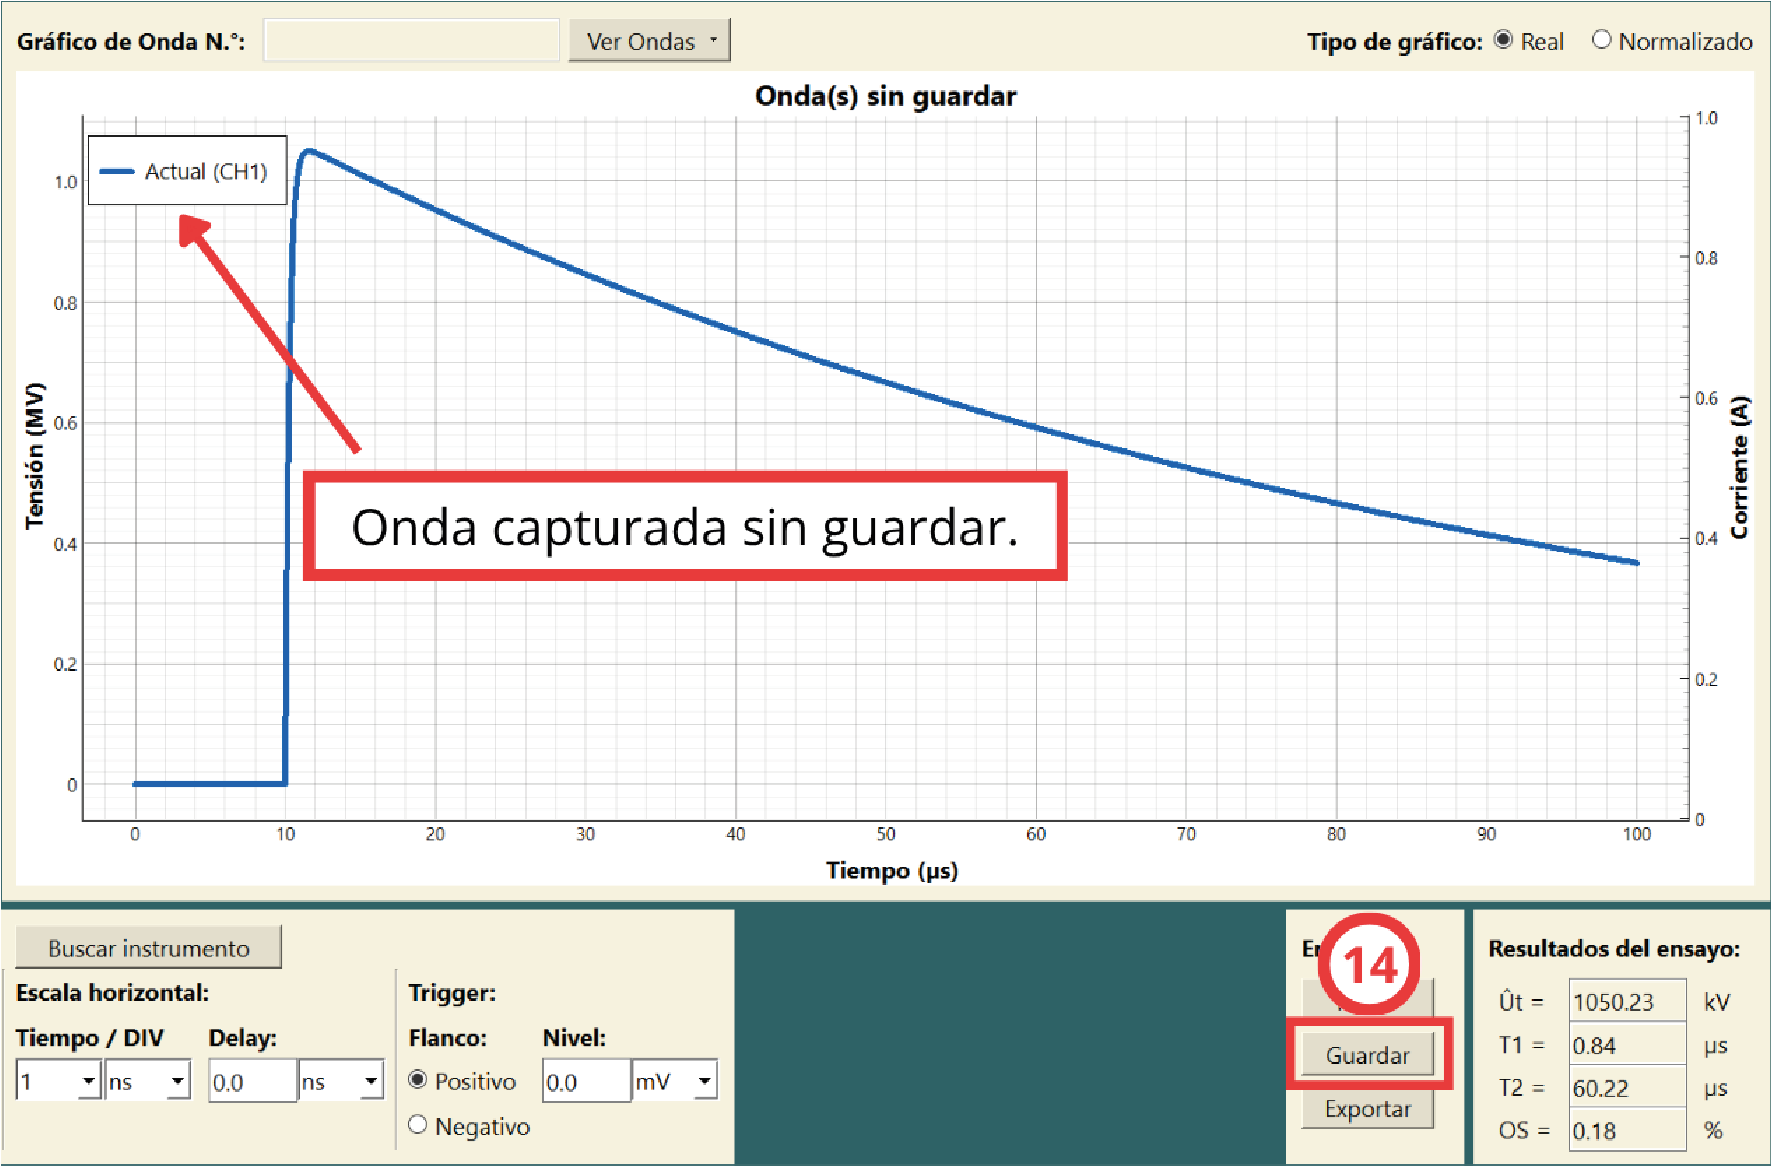
\includegraphics[width=1\textwidth]{img/GUI_uso_6_guardar_onda.png}
        \caption{Guardado de impulso.}
        \label{fig:GUI_uso_6_guardar_onda}
    \end{figure}
    \item [\textbf{Paso 14:}] Accionar el botón \enquote{Guardar}, para almacenar permanentemente la onda.
    \begin{figure}[H]
        \centering
        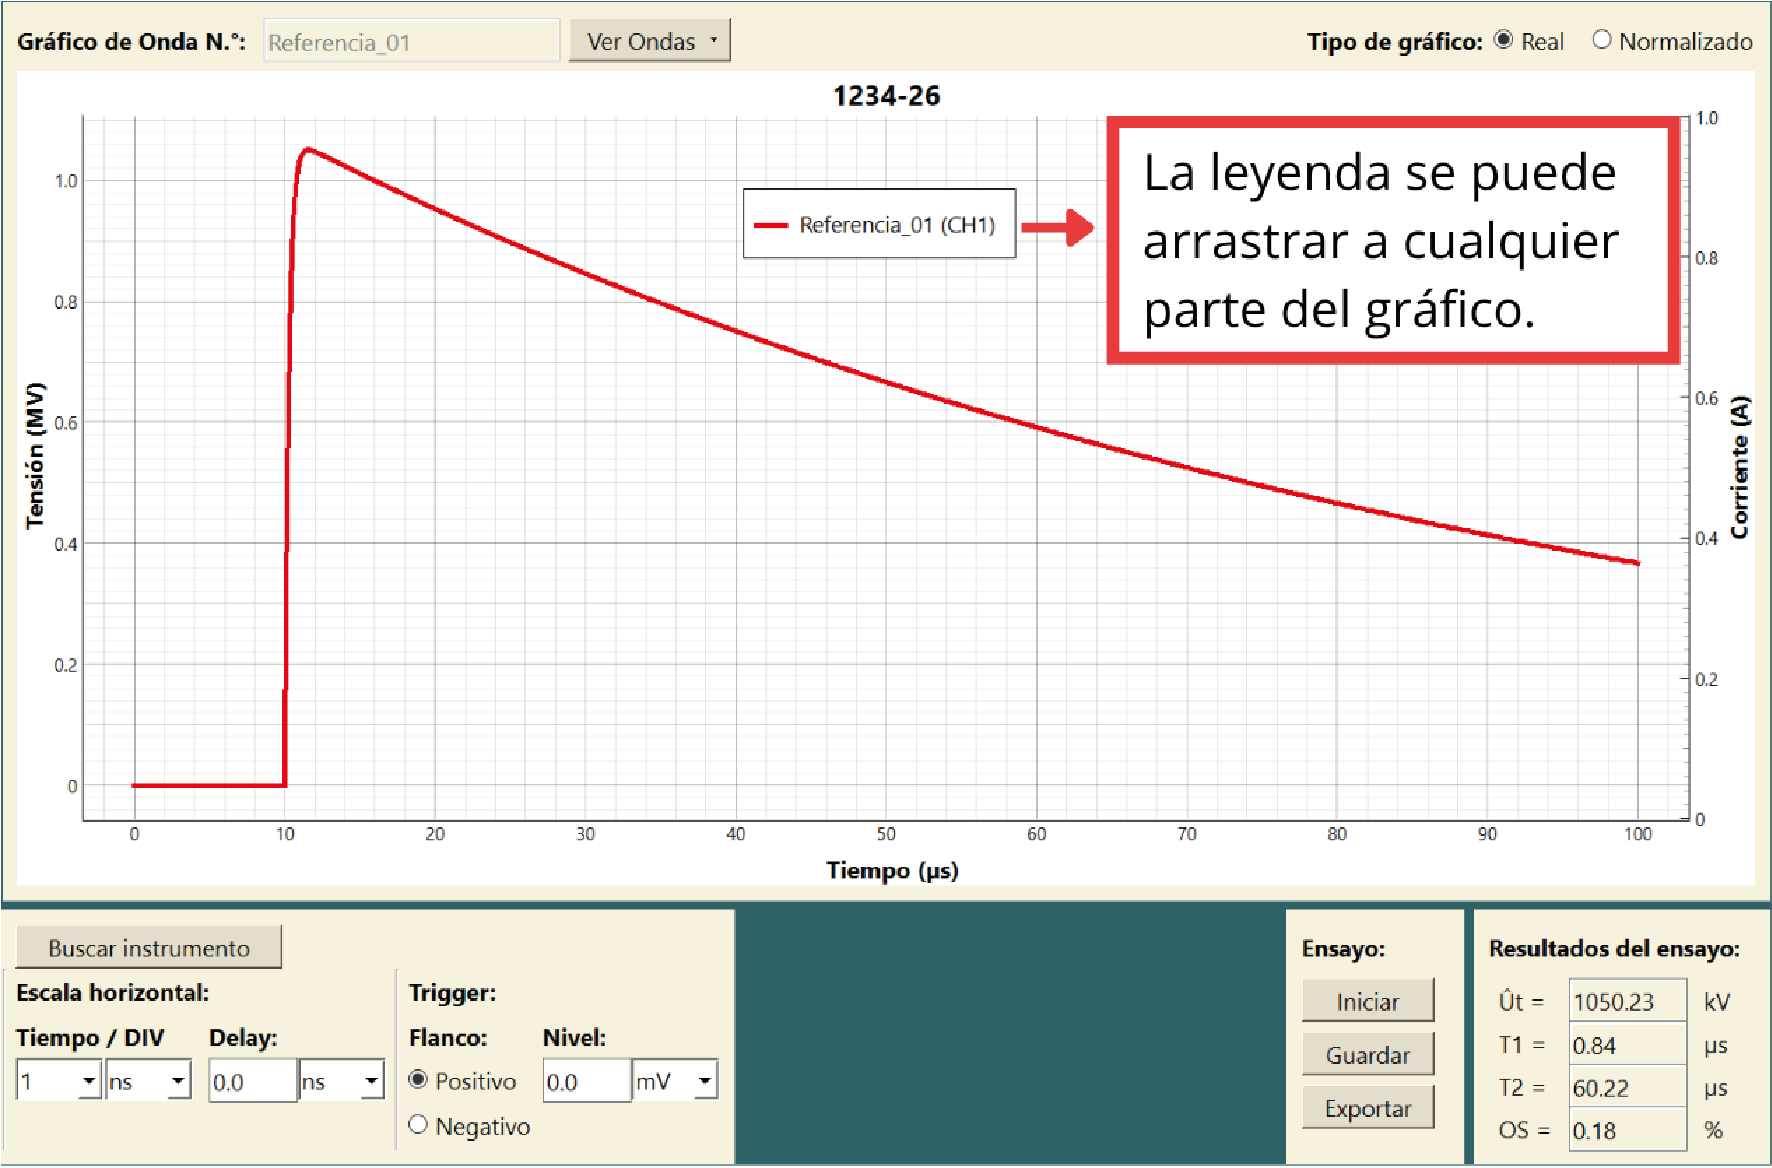
\includegraphics[width=1\textwidth]{img/GUI_uso_7_onda_guardada.png}
        \caption{Ejemplo de onda guardada.}
        \label{fig:GUI_uso_7_onda_guardada}
    \end{figure}
    Luego de guardar la onda, se puede mover la leyenda para que no interfiera con el gráfico. Y también, se puede ampliar/alejar el gráfico con la rueda el \emph{mouse}.
    \begin{figure}[H]
        \centering
        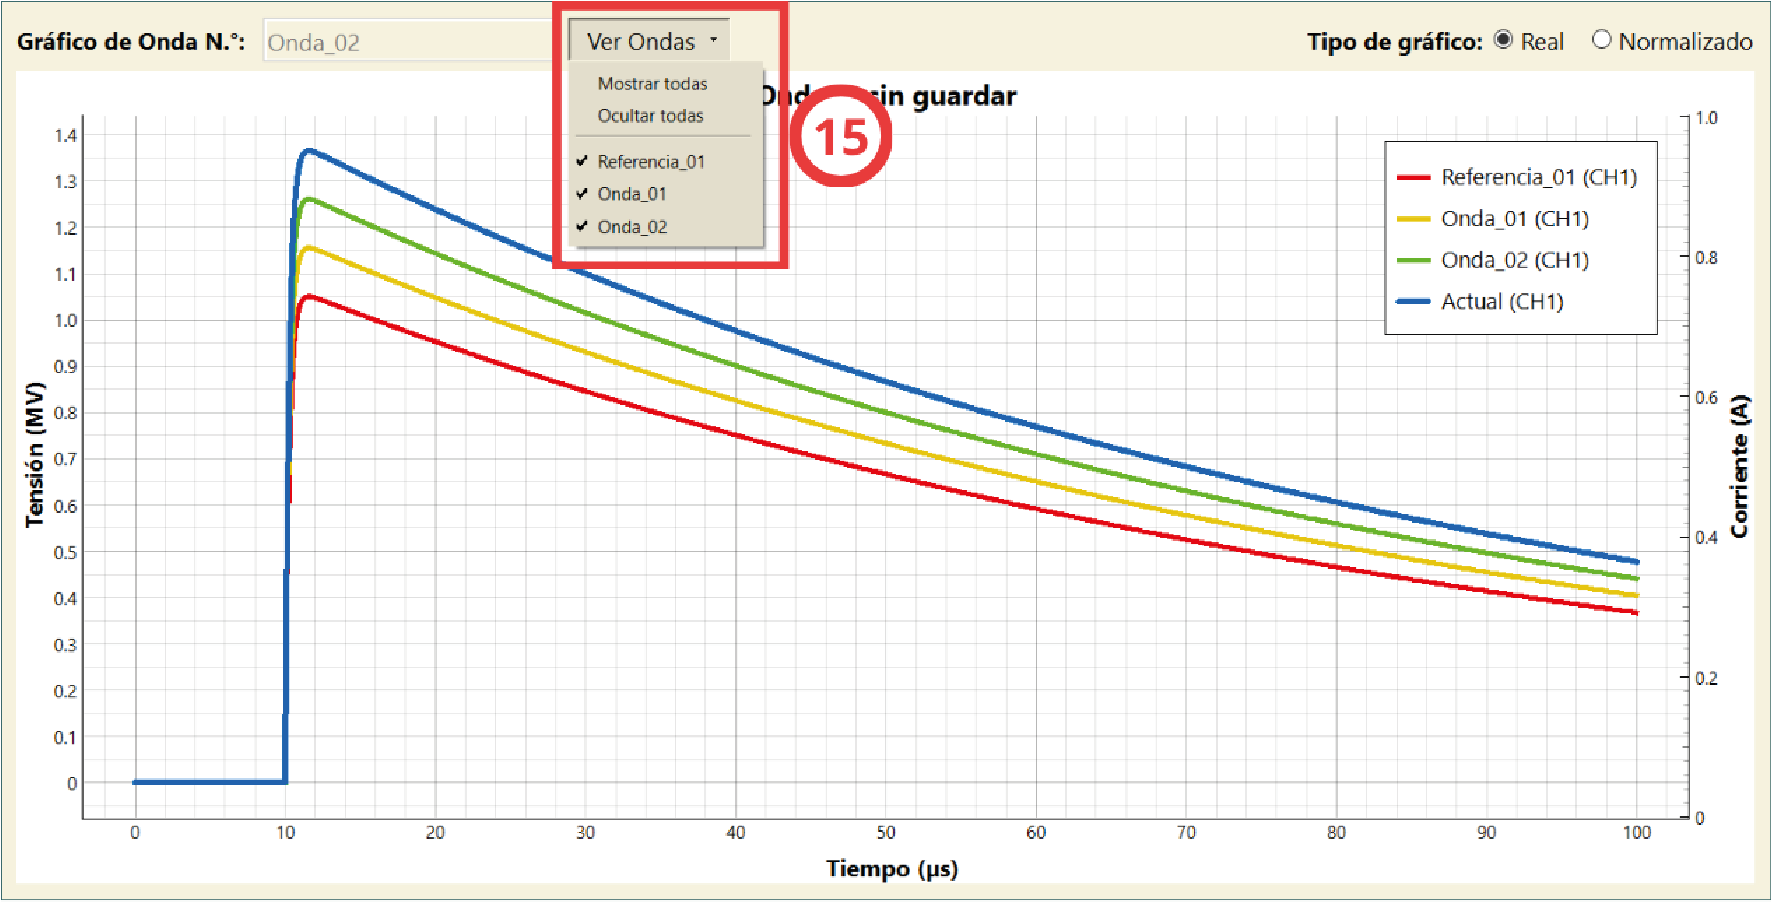
\includegraphics[width=1\textwidth]{img/GUI_uso_8_historial.png}
        \caption{Historial de impulsos guardados.}
        \label{fig:GUI_uso_8_historial}
    \end{figure}
    \item [\textbf{Paso 15:}] \textbf{(Opcional)} Accionar el botón \enquote{Ver Ondas} para ver el historial de ondas almacenadas. Donde se encuentran las opciones de mostrar/ocultar todas las ondas en simultáneo, o también se puede mostrar/ocultar individualmente cada una, seleccionando en la lista desplegable.
        \begin{figure}[H]
        \centering
        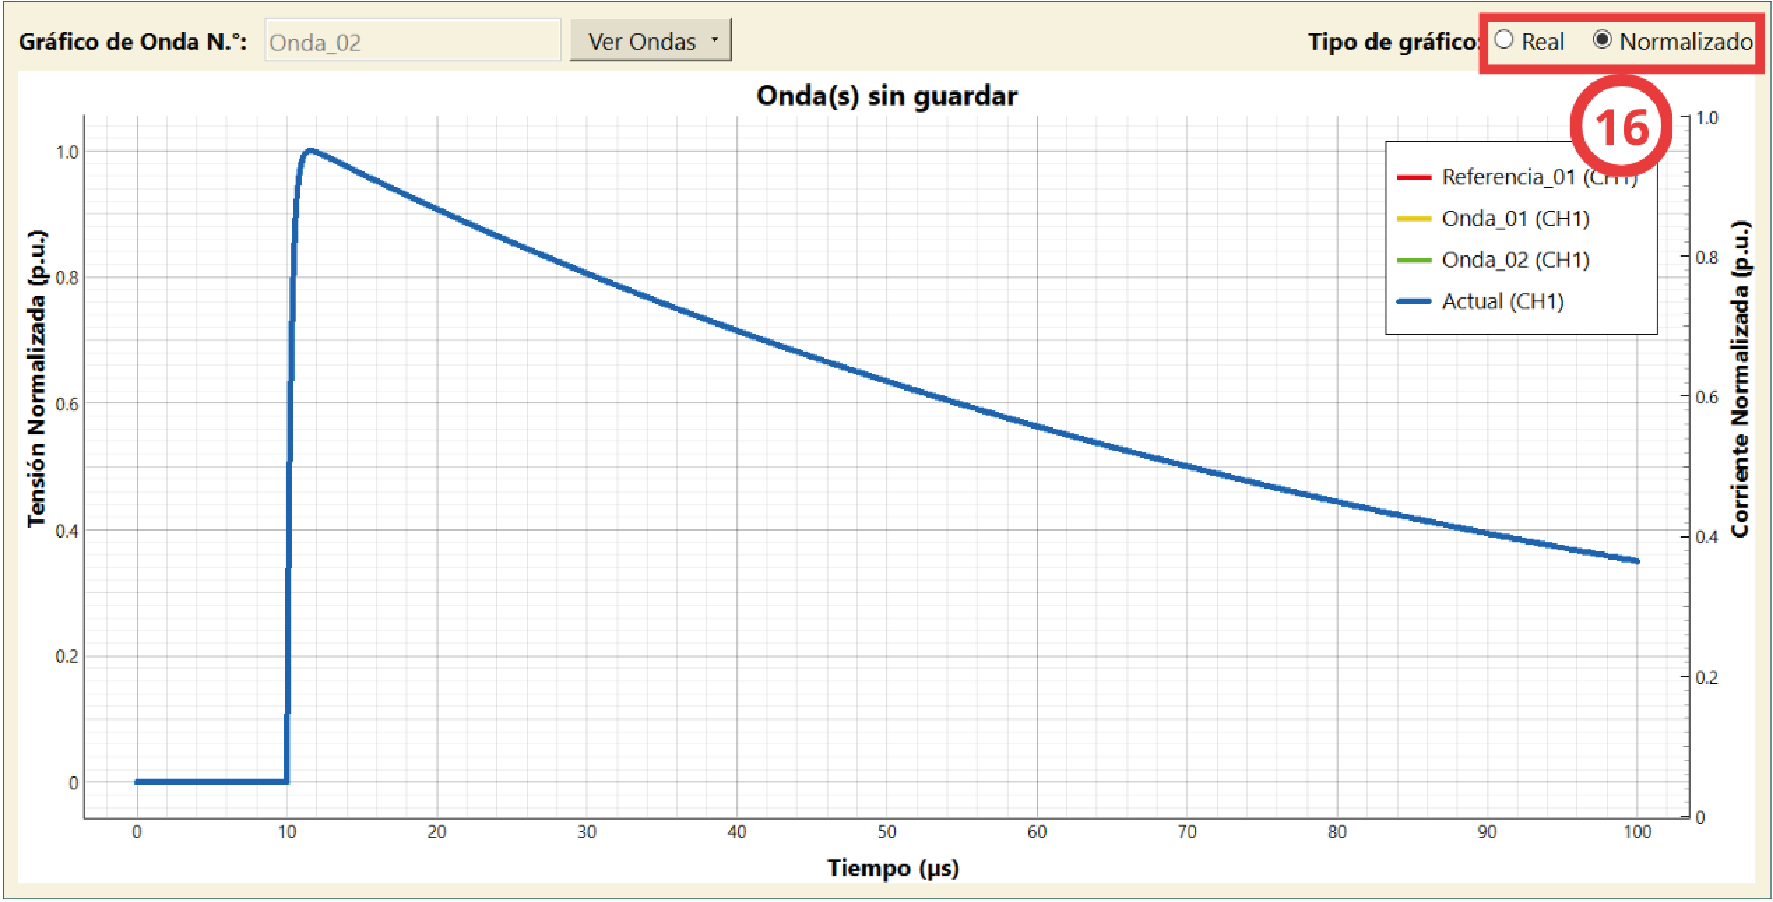
\includegraphics[width=1\textwidth]{img/GUI_uso_9_normalizar_ondas.png}
        \caption{Gráfico normalizado a valor unitario.}
        \label{fig:GUI_uso_9_normalizar_ondas}
    \end{figure}
    \item [\textbf{Paso 16:}] \textbf{(Opcional)} Accionar los botones de opciones \enquote{Real} o \enquote{Normalizado}, para ver las ondas en su magnitud real o escalada a valor unitario respectivamente.
        \begin{figure}[H]
        \centering
        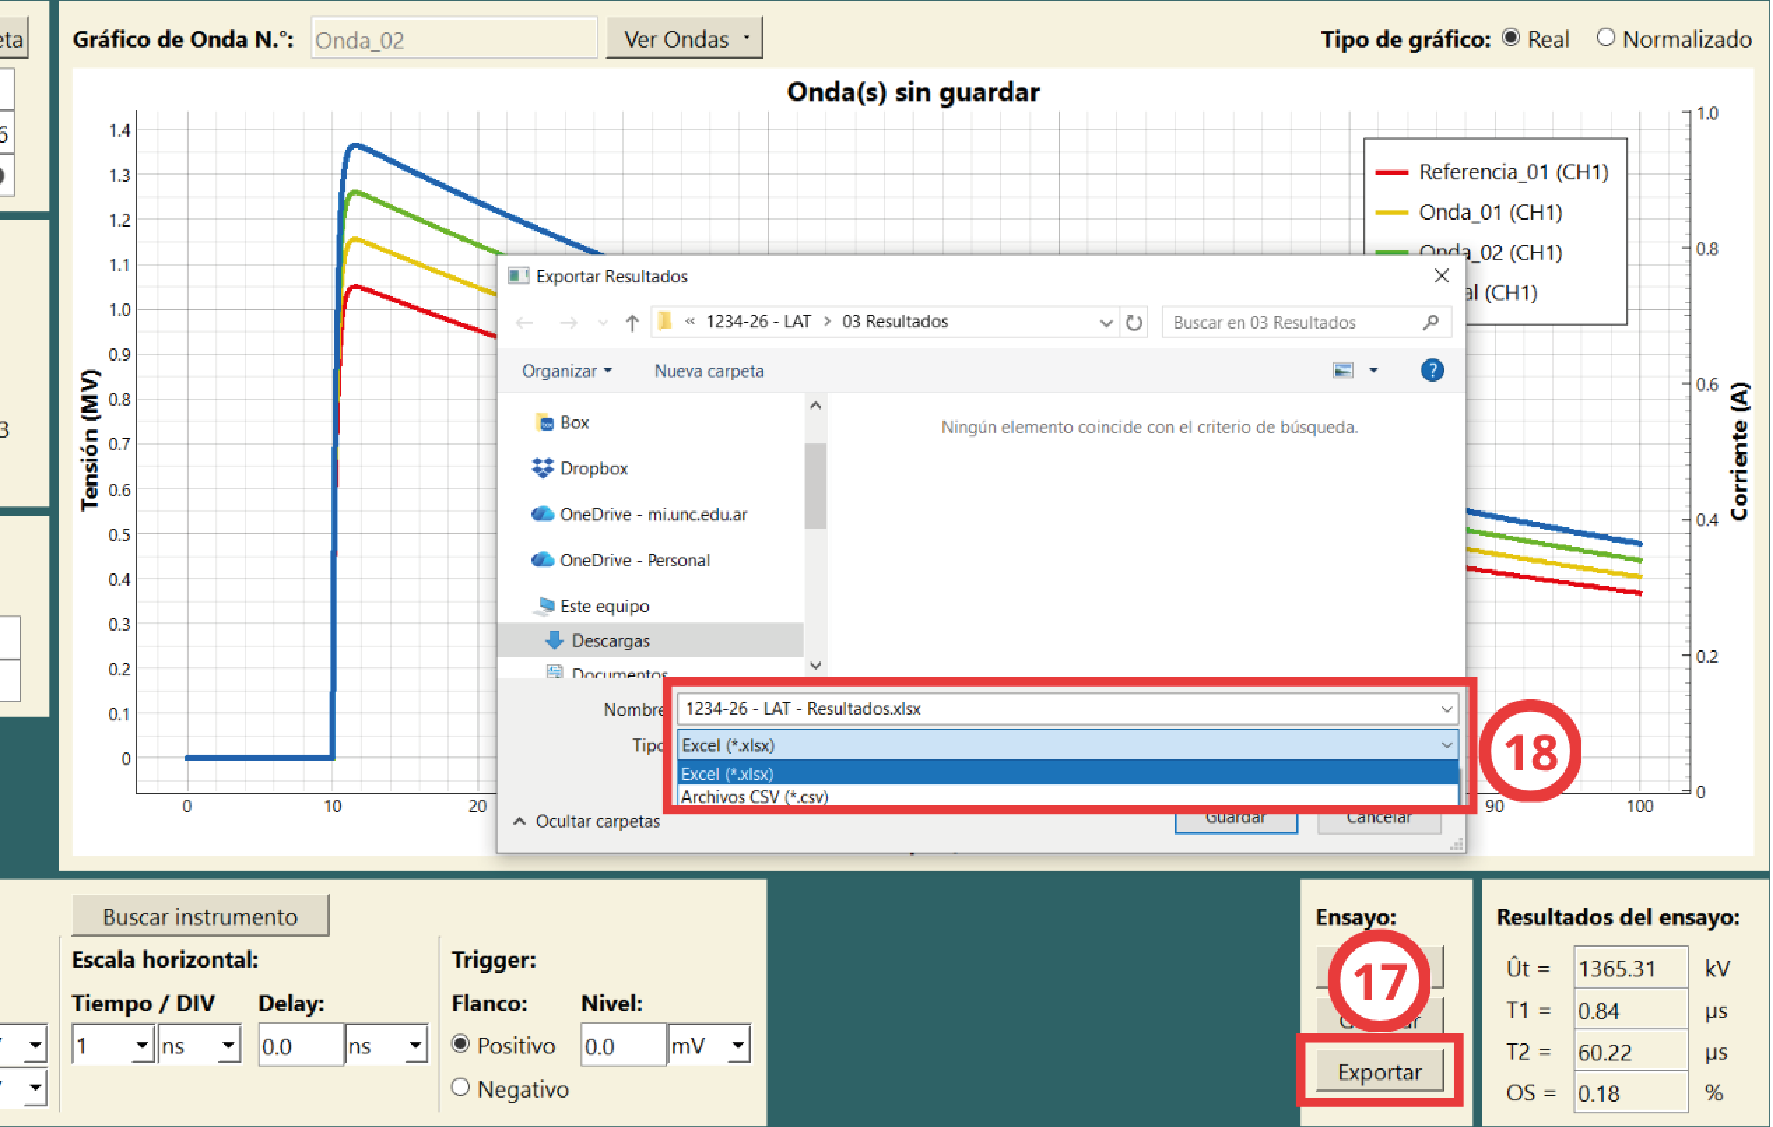
\includegraphics[width=1\textwidth]{img/GUI_uso_10_exportar.png}
        \caption{Ejemplo de exportación de resultados.}
        \label{fig:GUI_uso_10_exportar}
    \end{figure}
    \item [\textbf{Paso 17:}] Al finalizar la captura de impulsos, accionar el botón \enquote{Exportar}, para obtener los resultados en hojas de cálculo.
    \item [\textbf{Paso 18:}] Por defecto ya genera un nombre para el archivo saliente, pero puede modificarse. Luego, seleccionar el formato de salida deseado y accionar el botón \enquote{Guardar}.
\end{enumerate}